\documentclass[12pt,a4paper]{article}
\usepackage[utf8]{inputenc}
\usepackage[romanian]{babel}
\usepackage{graphicx}
\usepackage{amsmath}
\usepackage{amssymb}
\usepackage{geometry}
\usepackage{hyperref}
\usepackage{listings}
\usepackage{xcolor}
\usepackage{fancyhdr}
\usepackage[none]{hyphenat}
\usepackage{float}
\usepackage{enumitem}
\usepackage{titlesec}
\usepackage{tikz}
\usepackage{setspace} % Pentru distanța dintre rânduri
\usepackage{times} % Pentru font Times New Roman
\usepackage{algorithm}
\usepackage{algpseudocode}
\usepackage{algorithmicx}
\usepackage{csquotes}
\usepackage[backend=biber, style=numeric, sorting=ynt]{biblatex}
\addbibresource{bibliografie.bib}

\usetikzlibrary{arrows.meta, positioning, shapes.geometric}


% Eliminare redundanțe și avertismente

\geometry{
    a4paper,
    top=2.5cm,
    bottom=2.5cm,
    left=2.5cm,
    right=2.5cm
}

\hypersetup{
    colorlinks=true,
    linkcolor=blue,
    filecolor=magenta,      
    urlcolor=cyan,
}

% Stiluri pentru cod
\definecolor{codegreen}{rgb}{0,0.6,0}
\definecolor{codegray}{rgb}{0.5,0.5,0.5}
\definecolor{codepurple}{rgb}{0.58,0,0.82}
\definecolor{backcolour}{rgb}{0.95,0.95,0.92}

\lstdefinestyle{mystyle}{
    backgroundcolor=\color{backcolour},   
    commentstyle=\color{codegreen},
    keywordstyle=\color{magenta},
    numberstyle=\tiny\color{codegray},
    stringstyle=\color{codepurple},
    basicstyle=\ttfamily\footnotesize,
    breakatwhitespace=false,         
    breaklines=true,                 
    captionpos=b,                    
    keepspaces=true,                 
    numbers=left,                    
    numbersep=5pt,                  
    showspaces=false,                
    showstringspaces=false,
    showtabs=false,                  
    tabsize=2
}

\lstset{style=mystyle}


% Configurare text
\setstretch{1.5} % Distanța dintre rânduri
\setlength{\parindent}{0pt} % Eliminare indentare paragraf
\setlength{\parskip}{6pt} % Spațiu între paragrafe


\begin{document}

\begin{titlepage}
    \centering
    \begin{tabular}{p{2.5cm}p{10cm}p{2.5cm}}
    \includegraphics[width=2.5cm]{screenshots/s8.png} & 
    \begin{center}
    \vspace{-3.2cm}
    \textbf{Departamentul Automatică şi Informatică Industrială}\\
    \textbf{Facultatea Automatică şi Calculatoare}\\
    \textbf{Universitatea Nationala de Stiinta si Tehnologie}\\
    \textbf{POLITEHNICA din Bucureşti}\\
    Splaiul Independenţei 313, 060042, Bucureşti, România\\
    Sala ED 412, Tel. 021/402.92.69\\
    \href{http://www.aii.pub.ro}{www.aii.pub.ro}, email: secretariat.aii@upb.ro
    \end{center} & 
    \includegraphics[width=2.5cm]{screenshots/s9.png} \\
    \end{tabular}
    
    \vspace{3cm}
    
    {\Large\bfseries\centering Sesiunea de Comunicări Ştiinţifice Studenţeşti}

    {\large\bfseries\centering Ediţia 2025}

    \vspace{2cm}
    
    {\LARGE\bfseries\centering Sistem de Monitorizare Anti-Plagiat pentru Examene\\[2cm]}

    \vspace{\fill}
    
    \raggedright
    {\large\bfseries Autor: Valentin PLETEA-MARINESCU, Facultatea de Automatică și
    Calculatoare, anul 3, Grupa 332AB \par}
    {\large\bfseries Adresă email: pletea.valentin2003@gmail.com \par}
    {\large\bfseries Îndrumător ştiinţific: Conf. dr. ing. Ștefan Alexandru MOCANU\par}
\end{titlepage}

\hypersetup{linkcolor=black}
\tableofcontents
\newpage

\section{Introducere}

\subsection{Contextul și relevanța temei}

Plagiatul reprezintă una dintre problemele grave ale sistemului de
învățământ, iar, de când cu apariția și dezvoltarea inteligenței
artificiale, lucrurile s-au accentuat. Alegerea acestei teme constă în
oportunitatea de a oferi șanse egale tuturor participanților, în
cadrul unui examen, iar acest sistem de anti-plagiat, propus în acest
proiect, reprezintă o soluție inovatoare, prin combinarea tehnicilor
moderne de procesare a imaginilor și inteligență artificială\cite{russell2020artificial}, care își
propune să monitorizeze comportamentul candidaților și să semnaleze
posibile tentative de fraudă.

Utilizarea telefoanelor mobile ca instrument de înșelătorie în sălile de examinare a crescut
considerabil în ultimii ani, creând o povară suplimentară supraveghetorilor în asigurarea
integrității examenelor\cite{nazari2019detection}. Mai mult, studii recente în domeniul integrității
academice arată că plagiatul este „o abatere etică care afectează calitatea, lizibilitatea și
credibilitatea" rezultatelor academice, fiind esențială dezvoltarea de soluții pentru combaterea
practicilor inacceptabile\cite{zimba2021plagiarism}.

Conform studiului realizat de Gabriela Pelican\cite{pelican2021plagiat}, plagiatul
afectează absolut toate nivelurile educaționale, iar, în cazul
României, lucrurile nu merg foarte bine la capitolul acesta, autoarea
menționând că ``România prezintă cea mai ridicată rată a plagiatelor
descoperite pe tărâmul Uniunii, și anume 26.1\% din totalitatea
operelor verificate, valoare aproape dublă în comparație cu media
europeană, precum și aceea că incidența cazurilor de plagiat este cu
mult mai ridicată în statele din regiunea estică a Europei, țări ale
căror niveluri de trai și de educație sunt considerabil inferioare
raportat la țările vestice.''

De asemenea, un alt studiu\cite{brainard2018massive}, publicat de cei de la Science, ne
relatează că România este țara cu cel mai mare număr de articole
științifice eliminate din cuprinsul publicațiilor de specialitate ca
urmare a nerespectării normelor de conduită în cercetarea științifică,
prin raportare la totalul fondurilor alocate pentru cercetare și de
asemenea, ocupă locul secund în topul țărilor cu cel mai mare număr de
articole retrase raportat la totalul articolelor publicate, în urma
descoperirii plagierii.

\newpage

\subsection{Obiectivele proiectului}

Acest proiect își propune să ofere un sistem inovator pentru monitorizarea examenelor, cu următoarele obiective specifice:

\begin{enumerate}[label=\arabic*.]
    \item \textbf{Detecția privirii candidatului:} Semnalarea și înregistrarea situațiilor
    în care candidatul privește în alte direcții precum stânga, dreapta sau jos, 
    decât în propriul ecran al monitorului sau în propria foaie, în cazul unui examen scris.
    
    \item \textbf{Identificarea obiectelor neautorizate:} Detectarea dispozitivelor precum
    ceasuri inteligente sau telefoane, care pot fi folosite pentru a obține informații, 
    ceea ce ar duce la fraudarea respectivului examen.
    
    \item \textbf{Înregistrare și arhivare:} Realizarea unei înregistrări video în care 
    vor fi capturate și arhivate sesiunile de examen pentru o analiză ulterioară, 
    evidențiind tentativele probabile de fraudă.
    
    \item \textbf{Generarea rapoartelor:} Crearea rapoartelor detaliate în formate HTML, CSV și JSON,
    contribuind astfel la o analiză mai clară și mai sigură pentru evaluatori.
    
    \item \textbf{Interfață intuitivă:} Dezvoltarea unei interfețe grafice intuitive, care să permită
    supraveghetorilor utilizarea tuturor funcționalităților menționate anterior.
\end{enumerate}

\subsection{Avantajele abordării propuse}

În general, multe soluții de combatere a plagiatului se concentrează mai mult 
pe monitorizarea ecranului candidatului, dar acest sistem este centrat pe 
comportamentul fizic al acestuia. Consider că, prin urmărirea direcției privirii 
și detectarea obiectelor neautorizate, sistemul poate identifica indicii ale
comportamentului fraudulos, oferind dovezi concrete care pot fi analizate ulterior. 
Acest lucru poate contribui semnificativ la menținerea integrității academice, 
fără a mai fi nevoie să se creeze acea atmosferă de supraveghere excesivă.

Este normal ca respectivul sistem să ofere, pe lângă rezultatele
remarcabile, și falsuri pozitive, din cauza unor factori precum
iluminarea sălii de examen sau mișcări naturale ale capului, fără
intenția de a privi în altă direcție. Astfel, prin intermediul
funcționalităților de înregistrare video și semnalare în timp real a
comportamentelor posibil frauduloase, poate să existe, după terminarea
respectivului examen, o discuție între profesor și student pe baza
onestității sale și de a ajunge la rezultatul final. 

Tehnologia avansează pe zi ce trece, iar diversele tentative de plagiat se diversifică automat.
Așadar, este absolut firesc ca și sistemele care încearcă, prin
diverse mijloace, să combată fraudarea examenelor, să avanseze și ele.

\section{Analiza domeniului și soluții existente}

\subsection{Soluții similare existente pe piață}

Au apărut pe piață, de-a lungul timpului, diferite soluții de
monitorizare și combatere a fraudei în cadrul examenelor. În urma cercetării, am identificat
trei sisteme principale care propun soluții similare cu acest proiect: ProctorU\cite{proctoru}, 
Proctorio\cite{proctorio} și Respondus Lockdown Browser\cite{respondus}.

Recent, sisteme moderne de supraveghere online precum Honorlock au implementat tehnologii avansate 
care detectează utilizarea telefoanelor mobile „printr-o combinație de instrumente de supraveghere" și pot
determina când participanții încearcă să folosească dispozitive mobile neautorizate pentru a accesa 
conținut în timpul examenelor\cite{honorlock2023detecting}. De asemenea, cercetările recente în domeniul 
eye-tracking au propus „o soluție nouă de detectare a înșelăciunii în examene online prin utilizarea 
tehnologiei de urmărire a privirii"\cite{dilini2021cheating}, demonstrând eficacitatea acestei abordări
în detectarea comportamentelor suspecte.

\subsubsection{ProctorU}
ProctorU este una dintre cele mai utilizate platforme în
supravegherea examenelor online. Se bazează atât pe monitorizarea
ecranului candidatului, cât și pe comportamentul acestuia. 

\begin{table}[h]
\centering
\begin{tabular}{|p{7.5cm}|p{7.5cm}|}
\hline
\textbf{Puncte forte} & \textbf{Limitări} \\
\hline
\begin{itemize}
    \item Verificarea identității candidatului prin legitimație sau act de identitate
    \item Supravegherea umană în timp real
    \item Monitorizarea completă a activității pe calculator
    \item Detectarea comportamentului suspect prin AI
\end{itemize} & 
\begin{itemize}
    \item Costuri ridicate (15-25 USD per candidat)
    \item Necesită conexiune stabilă la internet
    \item Mai puțin adecvat pentru examenele fizice
    \item Probleme potențiale de confidențialitate
\end{itemize} \\
\hline
\end{tabular}
\caption{Analiza comparativă a sistemului ProctorU}
\end{table}

\newpage

Platforma înregistrează fiecare secundă, se asigură că nu există alte tab-uri
deschise, cu excepția aceluia în care se susține respectivul examen,
nu permite anumite combinații de taste din tastatură pentru funcții precum 
print, copy sau paste și, prin intermediul unei camere web, platforma poate 
supraveghea candidatul eficient.

\subsubsection{Proctorio}
Un alt sistem similar este Proctorio, asemănător cu
ProctorU, dar care este complet automatizat, întrucât se bazează doar
pe tehnologii de AI și învățare automată pentru detectarea posibilelor
tentative de fraudă, fără a mai avea nevoie de asistență umană.

\begin{table}[H]
\centering
\begin{tabular}{|p{7.5cm}|p{7.5cm}|}
\hline
\textbf{Puncte forte} & \textbf{Limitări} \\
\hline
\begin{itemize}
    \item Instalare și configurare simplă prin extensie browser
    \item Funcționalități de blocare a navigării web
    \item Algoritmi care reduc necesitatea intervenției umane
    \item Costuri mai reduse decât ProctorU
\end{itemize} & 
\begin{itemize}
    \item Rată ridicată de falsuri pozitive
    \item Dificultate în detectarea utilizării dispozitivelor secundare
    \item Funcționează doar pe Google Chrome
    \item Probleme de confidențialitate
\end{itemize} \\
\hline
\end{tabular}
\caption{Analiza comparativă a sistemului Proctorio}
\end{table}

Monitorizarea se bazează pe recunoaștere facială, analizând comportamentul prin 
intermediul mișcării capului sau a ochilor. Sistemul se ocupă și de monitorizarea 
ecranului, observă dacă există alte tab-uri deschise și dacă sunt pornite în fundal 
aplicații care ar putea facilita fraudarea examenului.

\subsubsection{Respondus Lockdown Browser}
Respondus Lockdown Browser reprezintă o abordare diferită, 
întrucât se concentrează pe crearea unui mediu securizat pentru examen,
prin blocarea accesului candidatului la alte aplicații și resurse.

Conform documentației sale oficiale\cite{respondus}, această soluție se
integrează cu sisteme de management al învățământului (LMS), precum Canvas,
Blackboard, Moodle, Schoology și Brightspace.

\begin{table}[H] % Changed from [h] to [H] to force table placement
    \centering
    \begin{tabular}{|p{7.5cm}|p{7.5cm}|}
    \hline
    \textbf{Puncte forte} & \textbf{Limitări} \\
    \hline
    \begin{itemize}
        \item Împiedicarea accesului la alte programe și resurse
        \item Integrare bună cu platforme educaționale (LMS)
        \item Costuri mai reduse comparativ cu alte soluții
        \item Ușor de implementat la nivel instituțional
    \end{itemize} & 
    \begin{itemize}
        \item Incapacitatea de a detecta dispozitive secundare
        \item Nu monitorizează comportamentul fizic al candidatului
        \item Funcționalitate restrânsă pe dispozitivele mobile
        \item Incompatibilitate cu programe specifice (IDE-uri, etc.)
    \end{itemize} \\
    \hline
    \end{tabular}
    \caption{Analiza comparativă a sistemului Respondus Lockdown Browser}
\end{table}

\subsection{Aspecte multimedia relevante}

\subsubsection{Protocoale și transmisie de date}
În cadrul aspectelor legate de multimedia, întâlnim protocoale care
asigură transmisia datelor sigură și optimizată:
\begin{itemize}
    \item \textbf{WebRTC} pentru comunicația audio-video în timp real. Acest protocol este utilizat pentru a transmite fluxul video capturat de la webcam către sistemul de procesare, asigurând o latență minimă și o calitate optimă a transmisiei\cite{sredojev2015webrtc}. În proiectul nostru, WebRTC este folosit pentru a permite monitorizarea în timp real a candidaților, oferind o conexiune stabilă și eficientă.
    \item \textbf{TLS/SSL} pentru criptarea întregului flux de date. Acest strat de securitate este esențial pentru a proteja datele transmise între client și server, prevenind accesul neautorizat sau interceptarea informațiilor sensibile\cite{yang2018tls}. În contextul proiectului nostru, TLS/SSL este utilizat pentru a securiza atât fluxul video, cât și datele generate, cum ar fi rapoartele de încălcări.

    Cu toate ca versiunea actuală a proiectului nostru se bazează pe procesare locală fără componente de comunicație în rețea, implementarea acestor tehnologii ar reprezenta o direcție valoroasă de dezvoltare viitoare, permițând monitorizarea la distanță a candidaților.
\end{itemize}

\subsubsection{Procesare video}
În ceea ce privește procesarea video, fluxul capturat de la webcam este procesat în timp real pentru a detecta comportamente suspicioase. Pentru salvarea înregistrărilor, sistemul nostru utilizează formate standard precum MP4, care incorporează codecul H.264, asigurând o eficiență bună în utilizarea spațiului de stocare\cite{goodfellow2016deep}.

Cercetările recente în domeniul sistemelor de supraveghere a examenelor au demonstrat eficiența detecției faciale și a urmăririi ochilor pentru identificarea comportamentelor suspecte\cite{alem2021novel}. Implementarea noastră se bazează pe aceste cercetări, integrând biblioteci precum \texttt{dlib} și \texttt{OpenCV} pentru a detecta poziția feței și direcția privirii, oferind astfel o soluție robustă pentru identificarea comportamentelor suspicioase.

Acest sistem se concentrează în principal pe analiza vizuală, detectând atât direcția privirii candidatului cât și prezența obiectelor neautorizate precum telefoanele mobile și ceasurile inteligente, elemente care reprezintă cele mai frecvente mijloace de fraudare în examene.
\subsubsection{Watermarking}
În soluțiile de tip Lockdown Browser se aplică watermark-uri vizibile sau invizibile asupra conținutului afișat pe ecran, cu scopul de a preveni capturarea neautorizată a informațiilor de examen. În proiectul nostru, watermark-urile sunt folosite pentru a marca fluxul video înregistrat cu informații precum data și ora reală, dar și valorile H și V, care indică in ce limite se afla direcția privirii candidatului. Acest tip de marcaj contribuie la asigurarea autenticității și integrității datelor înregistrate.

\subsubsection{Sincronizarea evenimentelor}
Pentru a asigura o corelare precisă între cadrele video și evenimentele detectate, proiectul nostru utilizează marcaje temporare. Acestea sunt generate în momentul capturării fiecărui cadru video și sunt utilizate pentru a lega alertele generate de sistem cu momentul exact al încălcării. Această abordare permite consultarea ulterioară a înregistrărilor video și verificarea eficientă a rapoartelor generate, oferind astfel dovezi concrete pentru evaluarea comportamentului candidatului în timpul examenului.
\subsubsection{Optimizări pentru resurse limitate}
Pentru a permite rularea eficientă a sistemului pe dispozitive cu resurse imitate, in acest sistem au fost implementate mai multe optimizări:
\begin{itemize}
    \item Procesarea unui cadru din 30 pentru detectarea obiectelor, reducând astfel consumul de resurse.
    \item Utilizarea unui buffer circular pentru gestionarea eficientă a cadrelor video.
    \item Integrarea unui sistem de cache pentru alertele generate, evitând duplicarea mesajelor de alertă.
\end{itemize}

\subsection{Avantajele soluției propuse față de cele existente}

Sistemul de monitorizare anti-plagiat dezvoltat în cadrul acestui proiect oferă numeroase beneficii comparative față de alternativele disponibile în prezent pe piață:

\begin{enumerate}
    \item \textbf{Monitorizare completă a comportamentului fizic} - În timp ce majoritatea soluțiilor comerciale (precum Proctorio sau Respondus) se limitează la supravegherea activității de pe ecranul calculatorului, sistemul nostru observă mișcările și gesturile candidatului. Această abordare permite detectarea unor tactici de fraudare care altfel ar trece neobservate, cum ar fi consultarea notițelor fizice sau comunicarea cu alte persoane prin gesturi. Sistemul analizează direcția privirii, orientarea capului și alte indicii fizice care pot semnala intenții frauduloase.
    
    \item \textbf{Identificarea precisă a dispozitivelor electronice neautorizate} - Prin implementarea algoritmilor YOLOv8 și a tehnicilor moderne de recunoaștere a obiectelor, aplicația noastră poate identifica cu acuratețe ridicată telefoane mobile, ceasuri inteligente și alte dispozitive folosite frecvent pentru înșelăciune. Această capabilitate depășește semnificativ funcționalitățile oferite de Respondus Lockdown Browser, care nu poate detecta utilizarea dispozitivelor secundare, și chiar și ale ProctorU, care se bazează în mare măsură pe supraveghetori umani pentru această sarcină.
    
    \item \textbf{Sistem avansat de raportare și documentare} - Aplicația generează automat rapoarte detaliate în formate versatile (HTML pentru vizualizare ușoară, CSV pentru analiză în Excel și JSON pentru integrare cu alte sisteme). Aceste rapoarte includ capturi de ecran cu momentele suspicioase, marcaje temporale precise și descrieri clare ale incidentelor, oferind evaluatorilor toate informațiile necesare pentru a lua decizii documentate. Sistemul păstrează astfel un istoric complet al sesiunii de examinare, permițând verificarea ulterioară și reducând disputele legate de posibilele sancțiuni.
    
    \item \textbf{Independență tehnologică și flexibilitate în implementare} - Acest sistem funcționează ca aplicație independentă, fără a fi constrâns de limitările specifice browserelor web sau platformelor online. Această arhitectură autonomă elimină dependențele externe și simplifică procesul de instalare și configurare la nivel instituțional. Natura sa independentă permite utilizarea pe o gamă largă de dispozitive și sisteme de operare, oferind instituțiilor educaționale libertatea de a implementa soluția fără a fi nevoite să adopte tehnologii sau servicii adiționale. Flexibilitatea sistemului facilitează adaptarea rapidă la cerințele specifice ale diferitelor tipuri de examene și contexte academice.
    
    \item \textbf{Eficiență economică și scalabilitate} - Implementarea locală a sistemului oferă avantaje semnificative din perspectiva costurilor pe termen lung. În timp ce multe soluții comerciale existente operează pe baza unui model de tarifare per student per examen, care poate deveni prohibitiv pentru instituțiile cu număr mare de studenți sau examene frecvente, aceasta propunere de sistem anit-plagiat necesită doar investiția inițială în infrastructura hardware existentă. Acest model scalabil permite instituțiilor educaționale să monitorizeze un număr nelimitat de examene fără costuri suplimentare, reducând costul efectiv per student cu fiecare sesiune organizată, iar această abordare face tehnologia de monitorizare anti-plagiat accesibilă inclusiv pentru instituțiile cu resurse financiare limitate.
    
    \item \textbf{Confidențialitate sporită a datelor studenților} - Prin procesarea locală a informațiilor, acest prototip elimină riscurile asociate cu transmiterea datelor către servere externe. Acest aspect este deosebit de important în contextul reglementărilor stricte privind protecția datelor personale, oferind instituțiilor control complet asupra informațiilor sensibile colectate în timpul examenelor.
\end{enumerate}

Combinația acestor avantaje face acest prototip de sistem anti-plagiat să reprezinte o soluție inovatoare și eficientă pentru asigurarea integrității academice, adaptată nevoilor actuale ale instituțiilor de învățământ.

\section{Arhitectura sistemului anti-plagiat}

Sistemul anti-plagiat dezvoltat reprezintă o soluție software complexă destinată monitorizării candidaților în timpul examenelor, cu scopul de a detecta și preveni comportamentele frauduloase. Arhitectura sistemului a fost concepută conform principiilor moderne de inginerie software, punând accent pe modularitate, extensibilitate și separarea clară a responsabilităților.

Baza dezvoltării sistemului este reprezenta de programarea orientată pe obiecte, care a permis structurarea aplicației în componente interconectate, fiecare având un rol bine definit în procesul de monitorizare. Această abordare facilitează nu doar dezvoltarea și testarea independentă a modulelor, ci și extinderea ulterioară a funcționalităților prin adăugarea de noi componente.

Sistemul prelucrează imaginile video pe măsură ce sunt captate, urmărind încotro se uită candidații și identificând obiecte nepermise cum ar fi telefoanele mobile și ceasurile inteligente. Această urmărire se bazează pe programe informatice care pot „vedea" și „înțelege" imaginile, organizate într-o structură pe niveluri care ține separate funcțiile simple de cele mai avansate.

Pentru a ilustra structura și funcționarea sistemului, am elaborat trei diagrame UML complementare: diagrama de clase, diagrama secvențială si diagrama de activitate. Aceste reprezentări oferă perspective diferite asupra arhitecturii, de la organizarea statică a claselor până la fluxurile dinamice de control și date.

\subsection{Diagrama de clase}

\begin{figure}[H]
    \centering
    \hspace{-2.7cm} % Added horizontal shift here before the tikzpicture
    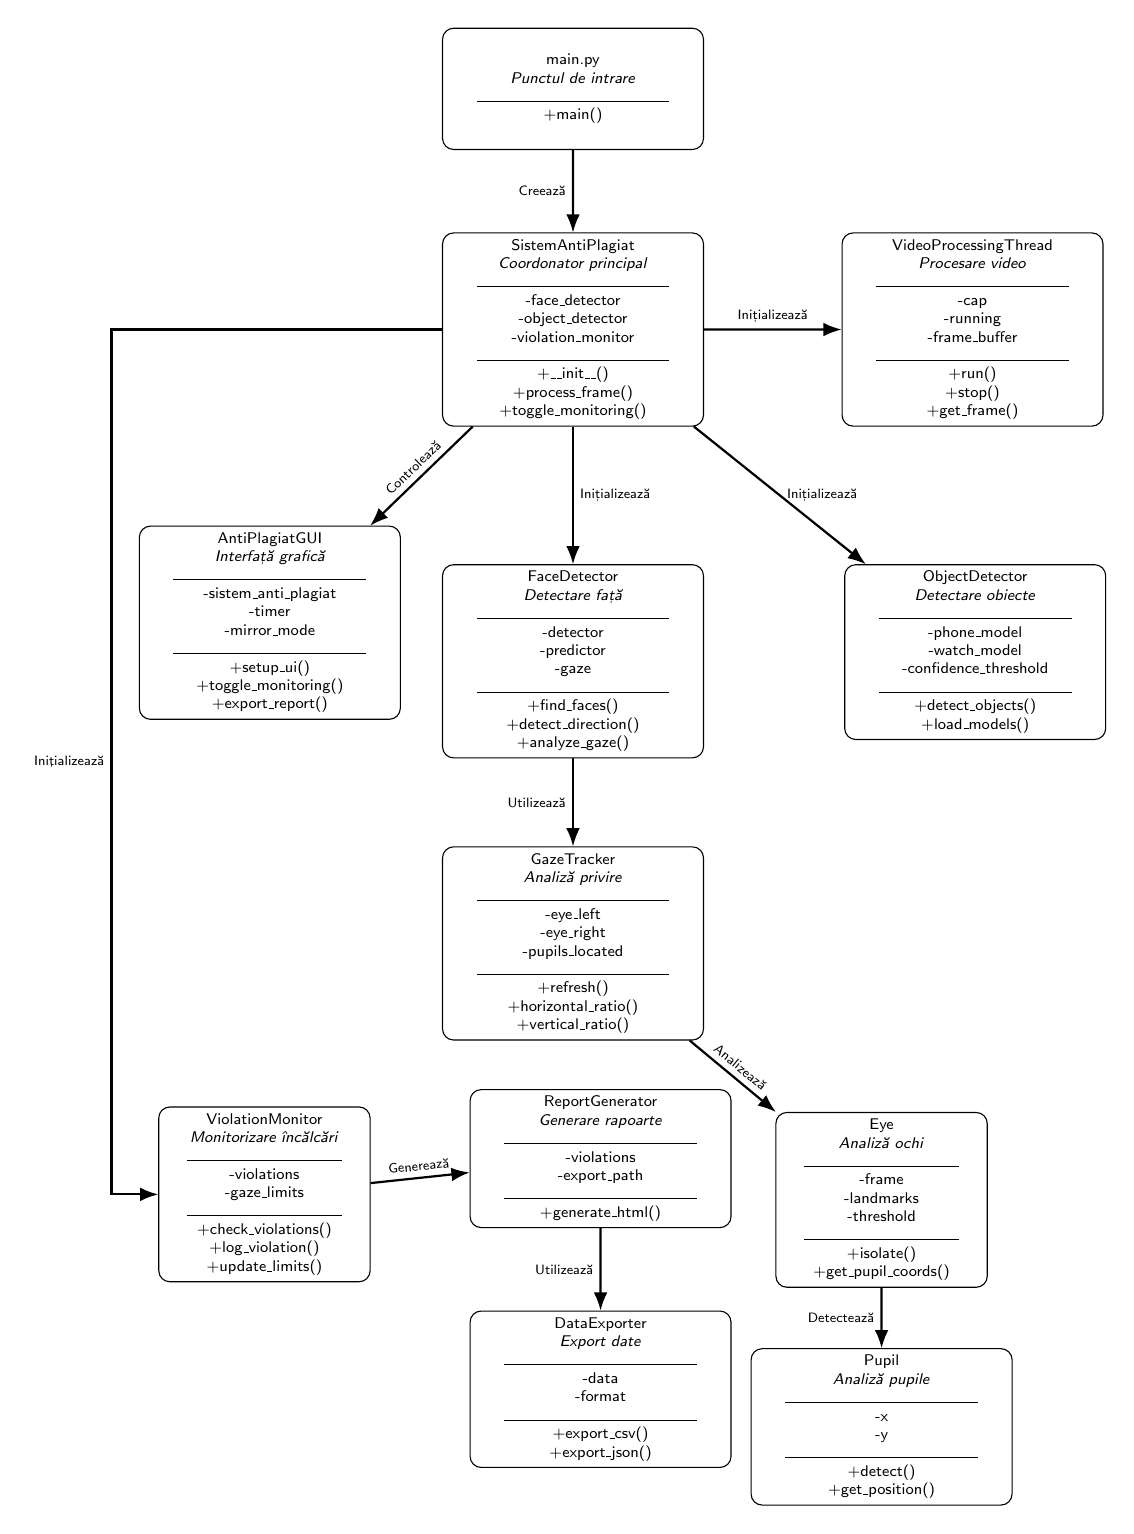
\begin{tikzpicture}[
        scale=0.7,
        transform shape,
        class/.style={rectangle, draw=black, rounded corners, text centered, text width=4.5cm, minimum height=2.2cm, font=\sffamily\footnotesize},
        smallclass/.style={rectangle, draw=black, rounded corners, text centered, text width=3.6cm, minimum height=1.8cm, font=\sffamily\footnotesize},
        relation/.style={-{Latex}, thick},
        shortrelation/.style={-{Latex}, thick, shorten >=2mm, shorten <=4mm},
        aggregation/.style={->, thick},
        composition/.style={->, thick},
        dependency/.style={dashed, ->, thick}
        ]
        % Classes with attributes and methods
        \node[class] (main) {main.py\\\textit{Punctul de intrare}\\\rule{3.5cm}{0.4pt}\\+main()};
        
        \node[class, below=1.5cm of main] (sistem) {SistemAntiPlagiat\\\textit{Coordonator principal}\\\rule{3.5cm}{0.4pt}\\-face\_detector\\-object\_detector\\-violation\_monitor\\\rule{3.5cm}{0.4pt}\\+\_\_init\_\_()\\+process\_frame()\\+toggle\_monitoring()};
        
        \node[class, below=1.8cm of sistem, xshift=-5.5cm] (gui) {AntiPlagiatGUI\\\textit{Interfață grafică}\\\rule{3.5cm}{0.4pt}\\-sistem\_anti\_plagiat\\-timer\\-mirror\_mode\\\rule{3.5cm}{0.4pt}\\+setup\_ui()\\+toggle\_monitoring()\\+export\_report()};
        
        \node[class, right=2.5cm of sistem] (video) {VideoProcessingThread\\\textit{Procesare video}\\\rule{3.5cm}{0.4pt}\\-cap\\-running\\-frame\_buffer\\\rule{3.5cm}{0.4pt}\\+run()\\+stop()\\+get\_frame()};
        
        \node[class, below right=2.5cm and -4.7cm of video] (object) {ObjectDetector\\\textit{Detectare obiecte}\\\rule{3.5cm}{0.4pt}\\-phone\_model\\-watch\_model\\-confidence\_threshold\\\rule{3.5cm}{0.4pt}\\+detect\_objects()\\+load\_models()};
        
        \node[class, below=2.5cm of sistem] (face) {FaceDetector\\\textit{Detectare față}\\\rule{3.5cm}{0.4pt}\\-detector\\-predictor\\-gaze\\\rule{3.5cm}{0.4pt}\\+find\_faces()\\+detect\_direction()\\+analyze\_gaze()};
        
        \node[class, below=1.6cm of face] (gaze) {GazeTracker\\\textit{Analiză privire}\\\rule{3.5cm}{0.4pt}\\-eye\_left\\-eye\_right\\-pupils\_located\\\rule{3.5cm}{0.4pt}\\+refresh()\\+horizontal\_ratio()\\+vertical\_ratio()};
        
        \node[smallclass, below left=1.2cm and 1.3cm of gaze] (violation) {ViolationMonitor\\\textit{Monitorizare încălcări}\\\rule{2.8cm}{0.4pt}\\-violations\\-gaze\_limits\\\rule{2.8cm}{0.4pt}\\+check\_violations()\\+log\_violation()\\+update\_limits()};
        
        \node[smallclass, below right=1.3cm and 1.3cm of gaze] (eye) {Eye\\\textit{Analiză ochi}\\\rule{2.8cm}{0.4pt}\\-frame\\-landmarks\\-threshold\\\rule{2.8cm}{0.4pt}\\+isolate()\\+get\_pupil\_coords()};
        
        \node[class, below =1.1cm of eye] (pupil) {Pupil\\\textit{Analiză pupile}\\\rule{3.5cm}{0.4pt}\\-x\\-y\\\rule{3.5cm}{0.4pt}\\+detect()\\+get\_position()};
        
        \node[class, below right=-3.5cm and 1.8cm of violation] (report) {ReportGenerator\\\textit{Generare rapoarte}\\\rule{3.5cm}{0.4pt}\\-violations\\-export\_path\\\rule{3.5cm}{0.4pt}\\+generate\_html()};
        
        \node[class, below=1.5cm of report] (exporter) {DataExporter\\\textit{Export date}\\\rule{3.5cm}{0.4pt}\\-data\\-format\\\rule{3.5cm}{0.4pt}\\+export\_csv()\\+export\_json()};

        % Relations
        \draw[relation] (main) -- (sistem) node[midway, left, font=\sffamily\scriptsize] {Creează};
        \draw[relation] (sistem) -- (gui) node[midway, above, sloped, font=\sffamily\scriptsize] {Controlează};
        \draw[relation] (sistem) -- (video) node[midway, above, sloped, font=\sffamily\scriptsize] {Inițializează};
        \draw[relation] (sistem) -- (face) node[midway, right, font=\sffamily\scriptsize] {Inițializează};
        \draw[relation] (sistem) -- (object) node[midway, right, font=\sffamily\scriptsize] {Inițializează};
        \draw[relation] (sistem.west) -- ++(-6,0) |- (violation.west) node[near start, left, font=\sffamily\scriptsize] {Inițializează};
        \draw[relation] (face) -- (gaze) node[midway, left, font=\sffamily\scriptsize] {Utilizează};
        \draw[relation] (gaze) -- (eye) node[midway, above, sloped, font=\sffamily\scriptsize] {Analizează};
        \draw[relation] (eye) -- (pupil) node[midway, left, font=\sffamily\scriptsize] {Detectează};
        \draw[relation] (violation) -- (report) node[midway, above, sloped, font=\sffamily\scriptsize] {Generează};
        \draw[relation] (report) -- (exporter) node[midway, left, font=\sffamily\scriptsize] {Utilizează};
        \end{tikzpicture}
        \caption{Diagrama de clase a sistemului Anti-Plagiat}
    \end{figure}

Diagrama de clase evidențiază organizarea ierarhică a modulelor sistemului anti-plagiat și relațiile dintre acestea. Punctul de intrare \texttt{main.py} creează instanța clasei \texttt{SistemAntiPlagiat}, care ocupă poziția centrală în arhitectură, coordonând toate celelalte componente. Săgeata de la \texttt{main.py} către \texttt{SistemAntiPlagiat} reprezintă această inițializare fundamentală de la care pornește întregul sistem.

\texttt{SistemAntiPlagiat} inițializează patru componente esențiale, reprezentate prin săgețile divergente: \texttt{AntiPlagiatGUI} pentru interfața grafică, \texttt{VideoHandler} pentru procesarea video, \texttt{FaceDetector} pentru analiza facială și \texttt{ObjectDetector} pentru identificarea obiectelor. Această structură reflectă metodele din constructorul clasei \texttt{SistemAntiPlagiat}, unde sunt create instanțele acestor obiecte.

Relația dintre \texttt{FaceDetector} și \texttt{GazeTracker} este una de creare, unde detectorul facial inițializează și utilizează modulul de urmărire a privirii. Această structură tip Facade simplifică interfața cu subsistemul complex de analiză a privirii. Observăm apoi cum \texttt{GazeTracker} utilizează \texttt{Eye} pentru izolarea regiunii oculare, care la rândul său folosește \texttt{Pupil} pentru localizarea precisă a pupilei. Această succesiune de delegări reflectă nivelul crescând de specializare a analizei.

\texttt{ViolationMonitor}, inițializat de \texttt{SistemAntiPlagiat}, agregă informațiile despre direcția privirii și obiectele detectate pentru a identifica comportamente suspecte. Când detectează încălcări, acestea sunt transmise către \texttt{ReportGenerator} care utilizează \texttt{DataExporter} pentru a salva rapoartele în diverse formate.

Această organizare reflectă principiul separării responsabilităților, fiecare clasă având un rol specific în analiza și procesarea datelor video pentru identificarea tentativelor de plagiat.

\subsection{Diagrama secvențială}

\begin{figure}[H]
    \centering
        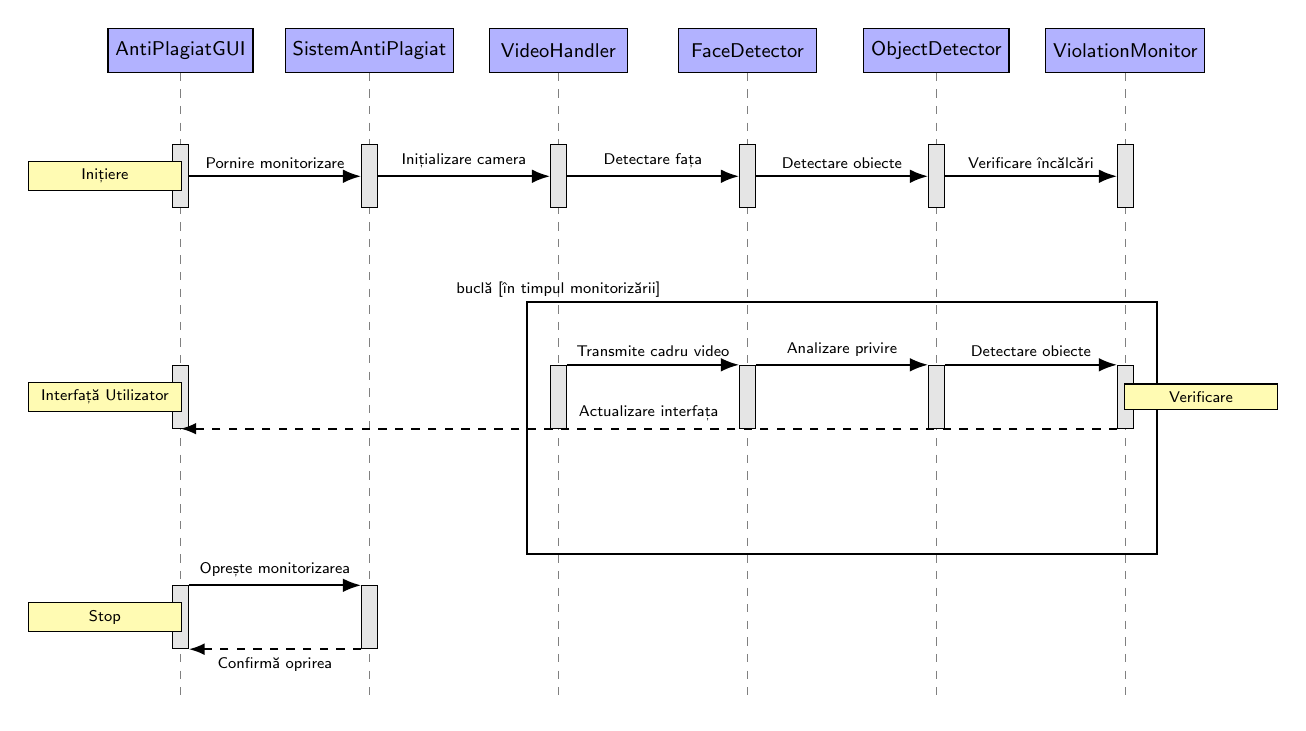
\begin{tikzpicture}[
                scale=0.8, % Reduced scale from 0.9 to 0.7
                transform shape,
                participant/.style={rectangle, draw=black, fill=blue!30, text centered, minimum width=2.2cm, minimum height=0.7cm, font=\sffamily\small},
                activation/.style={rectangle, draw=black, fill=gray!30, minimum width=0.25cm},
                lifeline/.style={dashed},
                message/.style={-{Latex}, thick},
                return/.style={-{Latex[length=2mm]}, dashed, thick},
                note/.style={rectangle, draw=black, fill=yellow!30, text width=2.2cm, text centered, font=\sffamily\scriptsize}
                ]
                % Participanți - aliniere pe orizontală cu spațiere redusă
                \node[participant] (gui) at (0,0) {AntiPlagiatGUI};
                \node[participant] (sistem) at (3,0) {SistemAntiPlagiat}; % Reduced from 3.5
                \node[participant] (video) at (6,0) {VideoHandler}; % Reduced from 7
                \node[participant] (face) at (9,0) {FaceDetector}; % Reduced from 10.5
                \node[participant] (object) at (12,0) {ObjectDetector}; % Reduced from 14
                \node[participant] (violation) at (15,0) {ViolationMonitor}; % Reduced from 17.5
                
                % Linii de viață
                \draw[lifeline, gray] (gui.south) -- +(0,-10); % Reduced from -12
                \draw[lifeline, gray] (sistem.south) -- +(0,-10);
                \draw[lifeline, gray] (video.south) -- +(0,-10);
                \draw[lifeline, gray] (face.south) -- +(0,-10);
                \draw[lifeline, gray] (object.south) -- +(0,-10);
                \draw[lifeline, gray] (violation.south) -- +(0,-10);
                
                % Bare de activare inițiale
                \node[activation, fill=gray!20] (gui_act1) at (0,-2) [minimum height=1cm] {}; % Reduced height
                \node[activation, fill=gray!20] (sistem_act1) at (3,-2) [minimum height=1cm] {};
                \node[activation, fill=gray!20] (video_act1) at (6,-2) [minimum height=1cm] {};
                \node[activation, fill=gray!20] (face_act1) at (9,-2) [minimum height=1cm] {};
                \node[activation, fill=gray!20] (object_act1) at (12,-2) [minimum height=1cm] {};
                \node[activation, fill=gray!20] (violation_act1) at (15,-2) [minimum height=1cm] {};
                
                % Mesaje inițiale
                \draw[message] (gui_act1) -- node[above, font=\sffamily\scriptsize] {Pornire monitorizare} (sistem_act1);
                \draw[message] (sistem_act1) -- node[above, font=\sffamily\scriptsize] {Inițializare camera} (video_act1);
                \draw[message] (video_act1) -- node[above, font=\sffamily\scriptsize] {Detectare fața} (face_act1);
                \draw[message] (face_act1) -- node[above, font=\sffamily\scriptsize] {Detectare obiecte} (object_act1);
                \draw[message] (object_act1) -- node[above, font=\sffamily\scriptsize] {Verificare încălcări} (violation_act1);
                
                % Buclă de procesare
                \draw[thick] (5.5,-4) rectangle (15.5,-8); % Reduced size
                \node[font=\sffamily\scriptsize] at (6,-3.8) {buclă [în timpul monitorizării]};
                
                % Activări în buclă
                \node[activation, fill=gray!20] (video_act2) at (6,-5.5) [minimum height=1cm] {};
                \node[activation, fill=gray!20] (face_act2) at (9,-5.5) [minimum height=1cm] {};
                \node[activation, fill=gray!20] (object_act2) at (12,-5.5) [minimum height=1cm] {};
                \node[activation, fill=gray!20] (violation_act2) at (15,-5.5) [minimum height=1cm] {};
                \node[activation, fill=gray!20] (gui_act2) at (0,-5.5) [minimum height=1cm] {};

                % Mesaje în buclă
                \draw[message] (video_act2.north east) -- node[above, font=\sffamily\scriptsize] {Transmite cadru video} (face_act2.north west);
                \draw[message] (face_act2.north east) -- node[above, font=\sffamily\scriptsize] {Analizare privire} (object_act2.north west);
                \draw[message] (object_act2.north east) -- node[above, font=\sffamily\scriptsize] {Detectare obiecte} (violation_act2.north west);
                \draw[return] (violation_act2.south west) -- node[above, font=\sffamily\scriptsize] {Actualizare interfața} (gui_act2.south);   % Secvența de stop
                \node[activation, fill=gray!20] (gui_act3) at (0,-9) [minimum height=1cm] {};
                \node[activation, fill=gray!20] (sistem_act2) at (3,-9) [minimum height=1cm] {};
                \draw[message] (gui_act3.north east) -- node[above, font=\sffamily\scriptsize] {Oprește monitorizarea} (sistem_act2.north west);
                \draw[return] (sistem_act2.south west) -- node[below, font=\sffamily\scriptsize] {Confirmă oprirea} (gui_act3.south east);
                
                % Note explicative - reduse și repoziționate
                \node[note] at (-1.2,-2) {Inițiere};
                \node[note] at (16.2,-5.5) {Verificare};
                \node[note] at (-1.2,-5.5) {Interfață Utilizator};
                \node[note] at (-1.2,-9) {Stop};
                
                \end{tikzpicture}
                \caption{Diagrama secvențială a sistemului Anti-Plagiat}
        \end{figure}

        Diagrama secvențială ilustrează interacțiunea temporală dintre componentele principale ale sistemului anti-plagiat. Secvența începe când utilizatorul inițiază monitorizarea prin interfața \texttt{AntiPlagiatGUI}, care transmite comanda către \texttt{SistemAntiPlagiat}. Acesta, la rândul său, inițializează camera prin \texttt{VideoHandler} și pornește procesele de detecție facială, detectare obiecte și monitorizare a încălcărilor.

        Bucla principală de procesare, evidențiată în diagramă, arată cum \texttt{VideoHandler} capturează cadre video care sunt apoi analizate de \texttt{FaceDetector} pentru poziția feței și direcția privirii, urmată de \texttt{ObjectDetector} pentru identificarea obiectelor interzise. \texttt{ViolationMonitor} primește rezultatele ambelor analize și determină dacă există încălcări, iar interfața grafică este actualizată corespunzător cu noile informații.

        Secvența se încheie cu oprirea monitorizării, când utilizatorul trimite comanda de stop prin interfață, iar sistemul confirmă încheierea procesului de monitorizare. Această succesiune de mesaje și activări ilustrează fluxul complet de control și date în sistem, de la inițiere până la încheiere, evidențiind modul în care toate componentele colaborează pentru a realiza monitorizarea în timp real a candidatului.


\subsection{Diagrama de activitate}

\begin{figure}[H]
    \centering
    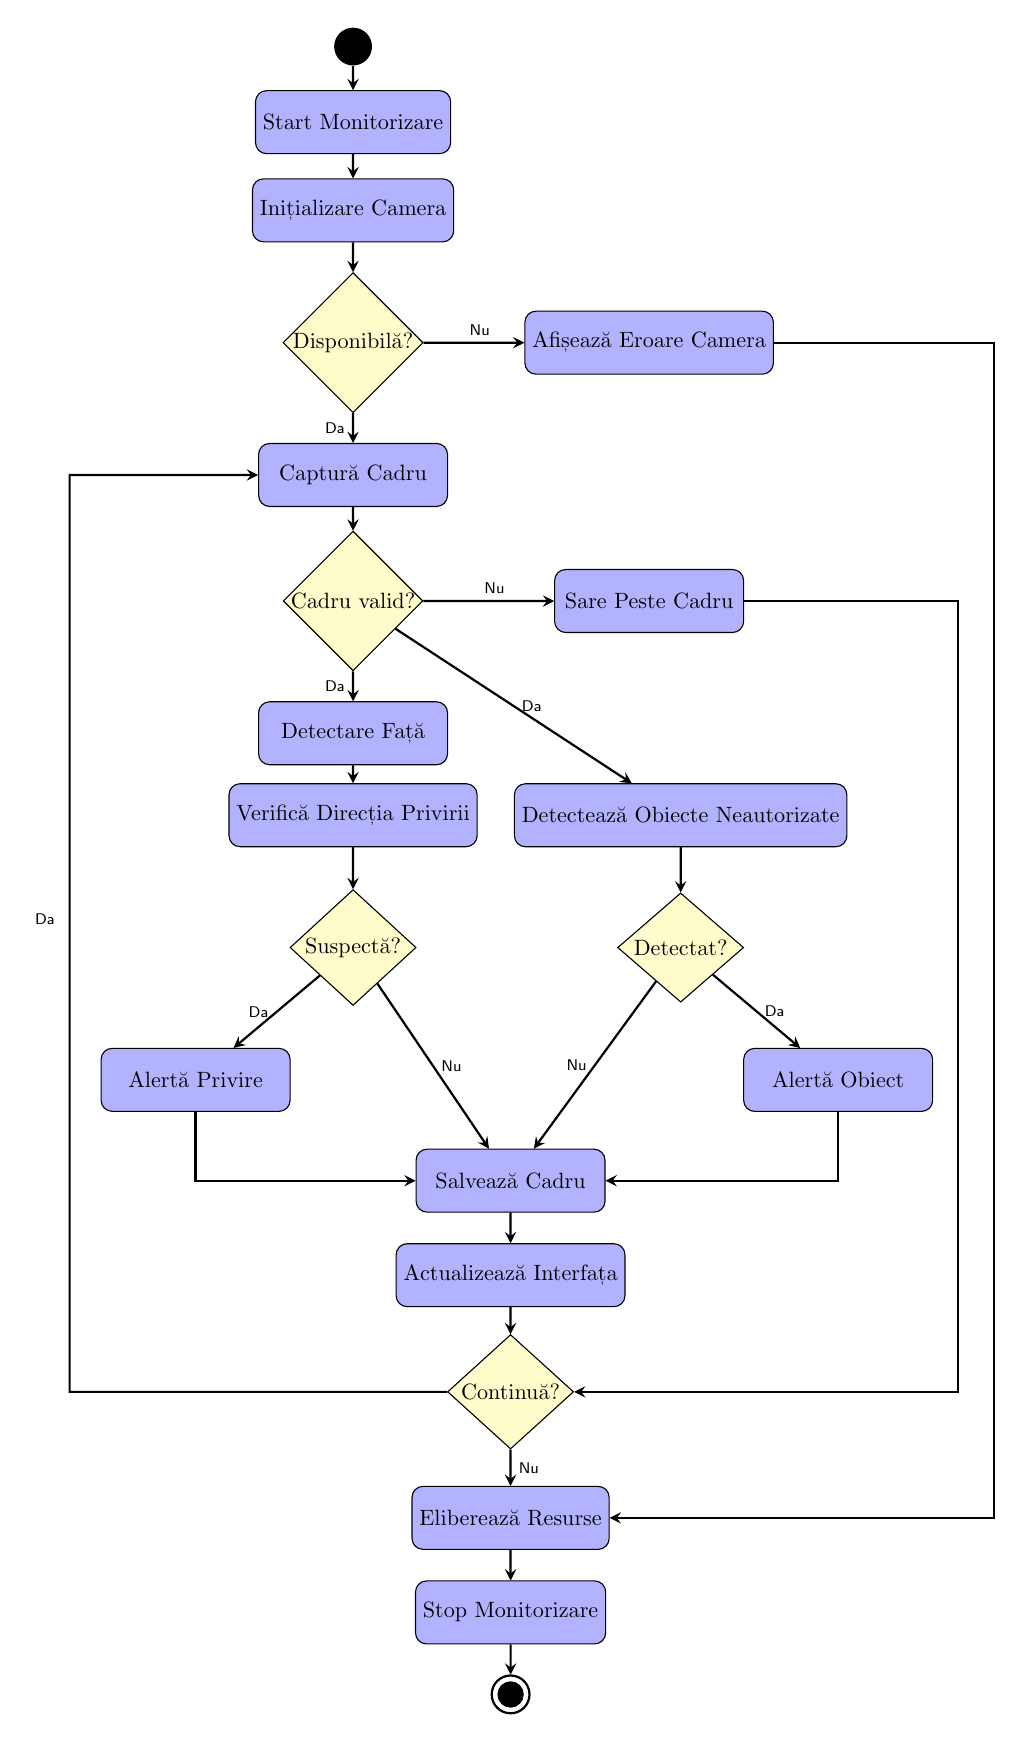
\begin{tikzpicture}[
        scale=0.8,
        transform shape,
        node distance=1.2cm,
        % Node styles
        start/.style={circle, fill=black, minimum width=0.6cm},
        end/.style={circle, draw=black, thick, fill=white, minimum width=0.6cm},
        process/.style={rectangle, draw=black, fill=blue!30, minimum width=3cm, 
                        minimum height=1cm, text centered, rounded corners},
        decision/.style={diamond, draw=black, fill=yellow!20, text centered, 
                        minimum width=2cm, minimum height=0.8cm, inner sep=0pt},
        arrow/.style={thick, ->, >=stealth}
    ]
        % Initial point and nodes
        \node[start] (initpoint) {};
        \node[process, below of=initpoint] (start) {Start Monitorizare};
        \node[process, below of=start, yshift=-0.2cm] (init) {Inițializare Camera};
        
        % New decision nodes for camera and frame validation
        \node[decision, below of=init, yshift=-0.9cm] (cameracheck) {Disponibilă?};
        \node[process, right of=cameracheck, xshift=3.5cm] (errorcamera) {Afișează Eroare Camera};
        
        \node[process, below of=cameracheck, yshift=-0.9cm] (capture) {Captură Cadru};
        \node[decision, below of=capture, yshift=-0.8cm] (framecheck) {Cadru valid?};
        \node[process, right of=framecheck, xshift=3.5cm] (errorframe) {Sare Peste Cadru};
        
        % Continue with original flow
        \node[process, below of=framecheck, yshift=-0.9cm] (face) {Detectare Față};
        
        % Split into two separate processes
        \node[process, below of=face, yshift=-0.1cm] (gazecheck) {Verifică Direcția Privirii};
        \node[process, right of=gazecheck, xshift=4.0cm] (objectcheck) {Detectează Obiecte Neautorizate};
        
        % Separate decision nodes
        \node[decision, below of=gazecheck, yshift=-0.9cm] (gazeviolation) {Suspectă?};
        \node[decision, below of=objectcheck, yshift=-0.9cm] (objectviolation) {Detectat?};
        
        % Separate alerts
        \node[process, below of=gazeviolation, xshift=-2.5cm, yshift=-0.9cm] (gazealert) {Alertă Privire};
        \node[process, below of=objectviolation, xshift=2.5cm, yshift=-0.9cm] (objectalert) {Alertă Obiect};
        
        % Continue flow
        \node[process, below of=gazeviolation, yshift=-2.5cm, xshift = 2.5cm] (save) {Salvează Cadru};
        \node[process, below of=save, yshift = -0.3cm] (update) {Actualizează Interfața};
        \node[decision, below of=update, yshift=-0.65cm] (continue) {Continuă?};
        \node[process, below of=continue, yshift=-0.8cm] (cleanup) {Eliberează Resurse};
        \node[process, below of=cleanup, yshift=-0.3cm] (stop) {Stop Monitorizare};
        
        % Draw end node with explicit inner black circle
        \node[end, below of=stop, yshift=-0.1cm] (endnode) {};
        \filldraw[black] (endnode.center) circle (0.2cm);
        
        % Arrows for initial flow
        \draw[arrow] (initpoint) -- (start);
        \draw[arrow] (start) -- (init);
        \draw[arrow] (init) -- (cameracheck);
        
        % Camera check paths
        \draw[arrow] (cameracheck) -- node[right, xshift=-0.2cm, yshift=+0.2cm, font=\sffamily\scriptsize] {Nu} (errorcamera);
        \draw[arrow] (cameracheck) -- node[left, font=\sffamily\scriptsize] {Da} (capture);
        \draw[arrow] (errorcamera.east) -- ++(3.5,0) |- (cleanup.east);
        
        % Frame check paths
        \draw[arrow] (capture) -- (framecheck);
        \draw[arrow] (framecheck) -- node[right, xshift=-0.2cm, yshift=+0.2cm, font=\sffamily\scriptsize] {Nu} (errorframe);
        \draw[arrow] (framecheck) -- node[left, font=\sffamily\scriptsize] {Da} (face);
        \draw[arrow] (framecheck) -- node[right, font=\sffamily\scriptsize] {Da} (objectcheck);
        \draw[arrow] (errorframe.east) -- ++(3.4,0) |- (continue.east);
        
        % Split path to two processes
        \draw[arrow] (face) -- (gazecheck);  
        
        % Decision paths
        \draw[arrow] (gazecheck) -- (gazeviolation);
        \draw[arrow] (objectcheck) -- (objectviolation);
        
        \draw[arrow] (gazeviolation) -- node[left, font=\sffamily\scriptsize] {Da} (gazealert);
        \draw[arrow] (objectviolation) -- node[right, font=\sffamily\scriptsize] {Da} (objectalert);
        
        % Join paths back
        \draw[arrow] (gazeviolation) -- node[right, font=\sffamily\scriptsize] {Nu} (save);
        \draw[arrow] (objectviolation) --node[left, font=\sffamily\scriptsize] {Nu} (save);
        \draw[arrow] (gazealert) |- (save);
        \draw[arrow] (objectalert) |- (save);
        
        % Continue flow
        \draw[arrow] (save) -- (update);
        \draw[arrow] (update) -- (continue);
        \draw[arrow] (continue) -- node[right, font=\sffamily\scriptsize] {Nu} (cleanup);
        \draw[arrow] (cleanup) -- (stop);
        \draw[arrow] (stop) -- (endnode);
        
        % Loop back to capture
        \draw[arrow] (continue) -- node[left, xshift=-3.1cm, yshift=7.5cm, font=\sffamily\scriptsize] {Da} ++(-7,0) |- (capture.west);
    \end{tikzpicture}
    \caption{Diagrama de activitate a sistemului Anti-Plagiat}
\end{figure}

Diagrama de activitate prezintă fluxul operațional al sistemului, evidențiind pașii procesării și punctele de decizie. Din starea inițială \texttt{Start Monitorizare}, activată când utilizatorul apasă butonul corespunzător, sistemul trece la \texttt{Inițializare Camera}, unde configurează parametrii de captură și verifică disponibilitatea camerei web. Această tranziție corespunde apelului metodei \texttt{toggle\_monitoring()} din clasa principală \texttt{AntiPlagiatGUI}.

După inițializare, sistemul verifică dacă respectiva cameră este disponibilă prin punctul de decizie \texttt{Disponibilă?}. În cazul unei erori, sistemul afișează un mesaj de eroare prin procesul \texttt{Afișează Eroare Camera} și avansează direct la eliberarea resurselor. Această verificare este implementată în metoda \texttt{VideoProcessingThread.run()}, unde se testează conexiunea la camera web.

Dacă aceasta este funcțională, procesul continuă cu \texttt{Captură Cadru}, unde se preiau cadre de la camera web. Sistemul validează apoi fiecare cadru capturat prin decizia \texttt{Cadru valid?}, care verifică dacă imaginea a fost obținută corect. Cadrele invalide sunt gestionate prin procesul \texttt{Sare Peste Cadru}, care le ignoră și continuă fluxul. Această verificare este implementată prin condiția \texttt{if ret and frame is not None} din modulul de procesare video.

După validarea cadrului, analiza se ramifică în două fluxuri paralele independente:

1. În primul flux, sistemul execută \texttt{Detectare Față}, unde \texttt{FaceDetector} localizează fața candidatului în imagine, urmată de \texttt{Verifică Direcția Privirii}, care analizează poziția reală a pupilelor pentru a determina în ce direcție privește candidatul, utilizând metoda \texttt{face\_detector.detect\_direction()}. La punctul de decizie \texttt{Suspectă?}, se evaluează dacă direcția privirii indică un comportament suspect (privire laterală sau în jos).

2. În paralel, în al doilea flux, \texttt{Detectează Obiecte Neautorizate} folosește modelele YOLOv8 pentru a scana imaginea și identifica telefoane sau ceasuri inteligente prin metoda \texttt{object\_detector.detect\_objects()}. Decizia \texttt{Detectat?} verifică prezența acestor obiecte interzise.

Aceste două fluxuri operează complet independent, procesând același cadru valid dar analizând aspecte diferite - unul concentrându-se pe comportamentul candidatului și altul pe mediul înconjurător. Această paralelizare reflectă arhitectura modulară a sistemului, unde \texttt{FaceDetector} și \texttt{ObjectDetector} funcționează ca module separate.

Fiecare flux poate genera alerte specifice când detectează potențiale încălcări: \texttt{Alertă Privire} pentru priviri suspecte și \texttt{Alertă Obiect} pentru obiecte neautorizate. Acestea sunt implementate prin apelul metodei \texttt{violation\_monitor.log\_violation()}, care înregistrează detaliile fiecărei încălcări.

Fluxurile converg apoi la activitatea \texttt{Salvează Cadru}, unde sistemul stochează imaginea procesată, urmată de \texttt{Actualizează Interfața}, care reîmprospătează display-ul cu datele analizate. Această actualizare este realizată prin semnalul \texttt{frame\_ready} din PyQt5, care declanșează actualizarea interfeței grafice.

La punctul de decizie \texttt{Continuă?}, sistemul evaluează dacă monitorizarea trebuie să continue. În caz afirmativ, procesul revine la \texttt{Captură Cadru} pentru o nouă iterație. În caz negativ, sistemul trece la \texttt{Eliberează Resurse}, unde se închid conexiunile la cameră și se eliberează memoria, urmată de \texttt{Stop Monitorizare}, când procesul se încheie oficial.

Această arhitectură robustă, cu procesare paralelă, permite sistemului să analizeze simultan diferite aspecte ale situației de examinare, crescând eficiența și precizia în detectarea tentativelor de fraudă, chiar și când una dintre metodele de analiză (detecția feței sau a obiectelor) ar putea întâmpina dificultăți temporare.

\section{Implementarea propriu-zisă}

În cadrul implementării sistemului de anti-plagiat, a fost necesară utilizarea mai multor biblioteci specializate, fiecare având un rol diferit în funcționarea sa.

\subsection{OpenCV}
Am utilizat biblioteca OpenCV (\texttt{Open Source Computer Vision Library}),
care a avut un rol principal în prelucrarea și procesarea imaginilor\cite{hasan2021face}. Cu
ajutorul ei, am captat fluxul video de la camera web, prin intermediul
funcției \texttt{VideoCapture}, care joacă rolul de interfață primară cu lumea
fizică, capturând imaginile candidatului care sunt apoi analizate pentru
a detecta comportamente suspecte.

Această bibliotecă mi-a oferit funcția \texttt{cvtColor}, cu care am reușit să
transform imaginile color în tonuri de gri, ceea ce a dus la o eficiență
mult mai mare pe partea de detectare facială, deoarece reduce
complexitatea computațională, făcând referire doar la o singură valoare
pentru fiecare pixel, în loc de trei, și îmbunătățește performanțele
algoritmilor de analiză a imaginii, care adesea funcționează mai bine cu
imagini în tonuri de gri.

În cadrul detecției precise al pupilelor, am aplicat un filtru gaussian,
cu scopul de a reduce zgomotul din imagini, apelând funcția
\texttt{cv2.GaussianBlur}, oferită de respectiva bibliotecă, care este un filtru
esențial în procesarea imaginilor. Parametrii acestei funcții sunt
imaginea sursă, fiind regiunea izolată a ochiului, dimensiunea
kernel-ului, în cazul nostru fiind de 7x7, deoarece s-a constatat, după
mai multe teste, că oferă cele mai bune rezultate pentru detectarea
pupilelor și este suficient de mare pentru a acoperi variațiile minore
de intensitate din jurul pupilei, în comparație cu kernel-uri mai mici
de 3x3 sau 5x5, care păstrează prea multe detalii fine și zgomot sau
kernel-uri prea mari de 9x9 sau 11x11, care estompează prea mult
imaginea, ducând la pierderea marginii pupilei și deviația standard a
distribuției Gaussiene, acest parametru fiind setat la valoarea 0,
însemnând că este calculată automat, folosind formula:

\begin{equation}
\sigma = 0.3 \cdot \left( \frac{\texttt{kernel\_size} - 1}{2} - 1 \right) + 0.8
\end{equation}

Pentru un kernel de dimensiune \(7 \times 7\), această formulă devine:
\begin{align}
\sigma &= 0.3 \cdot \left( \frac{7 - 1}{2} - 1 \right) + 0.8 \nonumber \\
    &= 0.3 \cdot (3 - 1) + 0.8 \nonumber \\
    &= 0.3 \cdot 2 + 0.8 \nonumber = 1.4
\end{align}

Funcția \texttt{cv2.minMaxLoc} din OpenCV este un instrument esențial pentru
detecția pupilelor. Această funcție identifică valorile minime și maxime
dintr-o imagine, împreună cu coordonatele acestora. Ea retunează patru
valori: valoarea minimă, valoarea maximă, coordonatele valorii minime și
coordonatele valorii maxime. În cazul nostru, valoarea de interes este
reprezentată de coordonatele valorii minime, deoarece reprezintă cel mai
întunecat punct din regiunea ochiului, iar pupila este tipic cea mai
întunecată parte a ochiului, deci această abordare eficientă permite
localizarea rapidă a centrului pupilei. Această metodă funcționează
deoarece, înainte de a aplica \texttt{minMaxLoc}, imaginea este pre-procesată de
acel filtru gaussian, menționat mai sus, care reduce zgomotul și
uniformizează valorile, făcând detectarea mai robustă la variații minore
în iluminare sau textura irisului.

\begin{figure}[H]
    \centering
    \includegraphics[width=0.5\textwidth]{screenshots/s5.png}
    \caption{Valori RGB ale pixelilor din zona oculară}
    \label{fig:rgb_ochi}
\end{figure}

Imaginea de mai sus reprezintă o captură de ecran a valorilor RGB ale
pixelilor din propria mea zona oculară, iar aceste rezultate au fost obtinute cu ajutorul rulării fisierului de testare \texttt{test\_camera.py}.


Tot cu ajutorul lui OpenCV, am reușit să desenez elemente vizuale
sugestive, cum ar fi dreptunghiuri în zona obiectelor detectate,
folosind funcția \texttt{cv2.rectangle()}, și să afișez text pentru alerte,
folosind \texttt{cv2.putText()}, iar salvarea și comprimarea înregistrărilor a
fost realizată folosind \texttt{VideoWriter}.

De asemenea, am reușit să creez o mască, pentru a izola obiectul de
interes, precum ochiul, utilizând funcții precum \texttt{fillPoly} și
\texttt{bitwise\_not}. Funcția \texttt{cv2.fillPoly} umple o zonă poligonală într-o imagine
cu o culoare specifică, iar, în contextul acestui sistem, este folosită
pentru a crea o mască pentru izolarea regiunii ochilor. Primește ca
parametrii imaginea pe care se desenează, un array de puncte care
definec poligonul, în cazul nostru fiind vorba de conturul ochiului, și
culoarea de umplere, spre exemplu (0, 0, 0), care în RGB înseamnă
culoare negru. Astfel, rezultatul este o mască în care regiunea ochiului
este colorată în negru, iar restul imaginii rămâne alb.

Funcția \texttt{cv2.bitwise\_not} inversează valorile de bit ale fiecărui pixel
din imagine, fiind echivalentă cu operația de negare bitwise ($\sim$). Am
folosit-o pentru a inversa masca creată, astfel încât regiunea ochiului
să fie izolată din restul imaginii. Această funcție primește ca
parametrii imaginea sursă și o mască opțională care determină pe ce
regiune se aplică operația. Astfel, aceste două funcții lucrează
împreună pentru a crea o ``tăietură'' precisă a regiunii ochiului, din
întreaga imagine, pentru a analiza foarte precis pupila, fără
interferențe din alte părți ale imaginii.

Funcția \texttt{cv2.circle} din OpenCV desenează un cerc pe o imagine, astfel eu
mă folosesc de aceasta, pentru evidențierea vizuală a pupilelor
detectate. Marchez poziția pupilelor detectate pe imagine, le evidențiez
utilizând culori diferite pentru a indica starea, precum verde pentru
privire centrată sau roșu pentru privire suspectă, și ofer în același
timp și un feedback vizual pentru supraveghetor, în ceea ce privește
direcția privirii candidatului. Ca și parametrii, funcția primește
imaginea pe care se desenează respectivul cerc, coordonatele centrului
cercului, în cazul nostru al centrului pupilei, raza cercului, culoarea
și grosimea liniei, dar, pentru grosime, am utilizat valoarea -1,
deoarece am vrut un cerc plin.

Așadar, biblioteca OpenCV este responsabilă pentru tot ce înseamnă ``a
vedea'' în acest sistem.

\subsection{Dlib}
Biblioteca Dlib a fost utilizată pentru detectarea feței și extragerea reperelor faciale\cite{el2023drowsiness}. Aceasta a fost esențială pentru analiza privirii și determinarea direcției acesteia. 

Funcția \texttt{dlib.get\_frontal\_face\_detector} a fost utilizată pentru a inițializa detectorul de fețe bazat pe HOG (Histogram of Oriented Gradients), care s-a dovedit eficient chiar și în condiții de iluminare variabilă. Acest algoritm funcționează prin împărțirea imaginii în celule mici și calcularea gradientului de intensitate pentru fiecare celulă. Gradientul este apoi normalizat pentru a reduce efectele variațiilor de iluminare, iar rezultatul este un descriptor robust care poate fi utilizat pentru a detecta fețele în imagine. Detectorul returnează coordonatele dreptunghiurilor care încadrează fețele detectate, iar aceste coordonate sunt utilizate pentru a izola regiunea feței.

Predictorul de repere faciale a fost încărcat cu ajutorul funcției \texttt{dlib.shape\_predictor}, care a permis identificarea celor 68 de puncte de pe față. Acest predictor utilizează un model preantrenat bazat pe regresie, care estimează pozițiile punctelor faciale pe baza caracteristicilor extrase din imagine. Dintre cele 68 de puncte, punctele 36-47 au fost utilizate pentru a izola regiunea ochilor. Aceste puncte sunt distribuite astfel încât să încadreze conturul ochilor, permițând izolarea precisă a regiunii de interes.

Funcția \texttt{shape.part} a fost utilizată pentru a accesa coordonatele fiecărui punct facial, iar aceste coordonate au fost folosite pentru a calcula raporturile orizontale și verticale ale privirii. De exemplu, raportul orizontal este calculat ca raportul dintre distanța dintre pupile și lățimea ochilor, iar raportul vertical este calculat ca raportul dintre înălțimea ochilor și lățimea acestora. Aceste raporturi sunt utilizate pentru a determina direcția privirii, cum ar fi privirea spre stânga, dreapta, sus sau jos.

De asemenea, aceste puncte au fost utilizate pentru a determina orientarea capului, prin calcularea distanțelor dintre punctele cheie, cum ar fi ochii, nasul și gura. Orientarea capului este estimată prin compararea acestor distanțe cu valorile de referință, iar rezultatul este utilizat pentru a detecta mișcările capului care pot indica comportamente suspecte.

\subsection{PyTorch și YOLOv8}
Pentru detectarea obiectelor interzise, precum telefoanele mobile și ceasurile inteligente, am utilizat biblioteca PyTorch\cite{pytorch} și modelul YOLOv8 dezvoltat de Ultralytics\cite{ultralytics}. 

Alegerea algoritmului YOLO pentru acest proiect este fundamentată pe cercetări academice recente care 
subliniază că „YOLO este adoptat în diverse aplicații în principal datorită inferențelor sale mai 
rapide"\cite{wang2022object}, făcându-l ideal pentru aplicații în timp real precum acest prototip. 
Acest algoritm „utilizează o rețea neuronală convoluțională profundă simplă pentru a detecta obiecte 
în imagine"\cite{v7labs2023yolo}, ceea ce îl face potrivit pentru detecția în timp real a obiectelor precum 
telefoanele sau ceasurile inteligente, chiar și în condiții de iluminare variabilă.

Funcția \texttt{torch.load} a fost utilizată pentru a încărca modelele YOLOv8 preantrenate. Aceste modele sunt bazate pe arhitectura YOLO (You Only Look Once), care este optimizată pentru detectarea rapidă și precisă a obiectelor în imagini\cite{redmon2018yolov3}. YOLOv8 utilizează o rețea neuronală convoluțională care împarte imaginea în grile și prezice simultan clasele obiectelor și coordonatele acestora. Această abordare permite detectarea în timp real, chiar și pe dispozitive cu resurse limitate.

Metoda \texttt{model.predict} a fost folosită pentru a detecta obiectele în cadrul video. Modelul a fost configurat să proceseze doar un cadru din 20 pentru a economisi resurse și să detecteze doar categoriile de interes. Această optimizare reduce semnificativ consumul de procesor și memorie, permițând rularea eficientă a aplicației pe hardware obișnuit.

Pentru a reduce falsurile pozitive, am utilizat două modele YOLOv8 separate: unul pentru detectarea telefoanelor și altul pentru ceasuri inteligente. Această abordare a permis clasificarea precisă a obiectelor detectate, chiar și în condiții de iluminare slabă sau când obiectele erau parțial vizibile. De exemplu, modelul pentru telefoane a fost antrenat să recunoască formele și dimensiunile tipice ale telefoanelor mobile, iar modelul pentru ceasuri inteligente a fost antrenat să detecteze dispozitivele purtabile pe încheietura mâinii.

Funcția \texttt{model.detect} a fost utilizată pentru a genera coordonatele obiectelor detectate, iar aceste coordonate au fost utilizate pentru a desena dreptunghiuri în jurul obiectelor și pentru a genera alerte în timp real. De asemenea, coordonatele au fost utilizate pentru a calcula distanțele dintre obiectele detectate și alte elemente din imagine, cum ar fi fața candidatului, pentru a determina dacă obiectele sunt utilizate în mod activ.

\subsection{NumPy}
Biblioteca NumPy a fost utilizată pentru manipularea matricelor și a datelor numerice\cite{harris2020array}. 

Funcția \texttt{np.zeros} a fost folosită pentru a crea măști pentru regiunile de interes din imagine, iar \texttt{np.full} a fost utilizată pentru a inițializa matrici cu valori constante. Aceste funcții sunt esențiale pentru preprocesarea imaginilor, deoarece permit izolarea regiunilor de interes și aplicarea de operații specifice doar asupra acestor regiuni\cite{goodfellow2016deep}.

Funcțiile \texttt{np.min} și \texttt{np.max} au fost utilizate pentru a determina limitele regiunilor de decupat, iar operațiile vectoriale au permis calcularea rapidă a coordonatelor pupilelor și a raporturilor orizontale și verticale. De exemplu, coordonatele pupilelor sunt calculate ca punctele cu intensitatea minimă din regiunea ochilor, iar raporturile sunt calculate ca raporturi între distanțele dintre aceste coordonate și dimensiunile regiunii.

\subsection{Datetime}
Biblioteca \texttt{datetime}\cite{pythondatetime} din Python a fost utilizată pentru gestionarea timpului și a marcajelor temporare în cadrul proiectului. Aceasta a fost esențială pentru sincronizarea evenimentelor, generarea rapoartelor și înregistrarea timpului de monitorizare.

Funcția \texttt{datetime.now()} a fost folosită pentru a obține timpul curent în momentul generării unui eveniment, cum ar fi detectarea unei nereguli si salvarea unui raport. Marcajele temporare create sunt utilizate pentru a lega evenimentele detectate de momentele exacte din fluxul video.

De exemplu, în cadrul clasei \texttt{ViolationMonitor}, funcția \texttt{datetime.now().strftime()} a fost utilizată pentru a formata marcajele temporare într-un format ușor de citit, cum ar fi \texttt{YYYY-MM-DD HH:MM:SS}. Acestea sunt incluse în rapoartele generate și sunt utilizate pentru a analiza comportamentul candidatului în timp.

Funcția \texttt{timedelta} a fost utilizată pentru a calcula diferențele de timp între evenimente. De exemplu, timpul scurs de la începutul înregistrării este calculat utilizând \texttt{datetime.now()} și timpul de start al înregistrării. Acest lucru este afișat în interfața grafică pentru a oferi utilizatorului informații în timp real despre durata monitorizării.

De asemenea, biblioteca \texttt{datetime} a fost utilizată pentru a genera nume unice pentru fișierele de înregistrare și rapoarte, utilizând funcția \texttt{strftime()} pentru a include marcaje temporare în numele fișierelor.

Biblioteca \texttt{datetime} a fost astfel un instrument esențial pentru gestionarea timpului în toate aspectele proiectului, de la monitorizare în timp real până la generarea rapoartelor detaliate.

\subsection{Logging}
Biblioteca \texttt{logging}\cite{pythonlogging} din Python a fost utilizată pentru gestionarea mesajelor de jurnalizare (\textit{logging}) în cadrul proiectului. Aceasta a fost esențială pentru monitorizarea funcționării aplicației, diagnosticarea problemelor și păstrarea unui istoric al evenimentelor importante.

Funcția \texttt{logging.basicConfig()} a fost utilizată pentru a configura formatul și nivelul de jurnalizare. În cadrul proiectului, mesajele de jurnalizare sunt salvate atât într-un fișier (\texttt{sistem\_anti\_plagiat.log}), cât și afișate în consolă. Acest lucru permite o monitorizare eficientă a aplicației în timp real, precum și o analiză ulterioară a problemelor.

De exemplu, în cadrul clasei \texttt{SistemAntiPlagiat}, biblioteca \texttt{logging} a fost utilizată pentru a înregistra evenimente importante, cum ar fi pornirea înregistrării video, detectarea încălcărilor sau erorile apărute în timpul procesării.

Biblioteca \texttt{logging} a fost utilizată și pentru a înregistra excepțiile apărute în timpul rulării aplicației, utilizând funcția \texttt{logger.exception()}, care include automat detaliile despre excepție în mesajul de jurnalizare.

Această abordare a permis identificarea rapidă a problemelor și îmbunătățirea stabilității aplicației. Biblioteca \texttt{logging} a fost astfel un instrument esențial pentru gestionarea mesajelor de jurnalizare în toate modulele proiectului.

\subsection{PyQt5}
Pentru dezvoltarea interfeței grafice, am utilizat biblioteca PyQt5\cite{pyqt5}. Aceasta a permis crearea unei interfețe intuitive și funcționale, utilizând următoarele componente principale:

\begin{itemize}
    \item \textbf{QPushButton:} Am folosit acest widget pentru a crea butoane interactive, cum ar fi cele pentru pornirea monitorizării, înregistrării sau exportarea rapoartelor. Aceste butoane sunt esențiale pentru a permite utilizatorului să interacționeze cu aplicația într-un mod simplu și direct. De exemplu, butonul de export al raportului oferă o funcționalitate clară și accesibilă pentru utilizator.

    \item \textbf{QTextEdit:} Acest widget este utilizat pentru afișarea în timp real a rapoartelor generate. Este o alegere potrivită deoarece permite afișarea unui text formatat și poate fi setat ca "read-only", astfel încât utilizatorul să nu poată modifica conținutul raportului.

    \item \textbf{QTimer:} Timer-ul este folosit pentru actualizarea periodică a timpului de înregistrare. Aceasta este o soluție eficientă pentru a menține interfața sincronizată cu procesele din fundal, cum ar fi monitorizarea în timp real.

    \item \textbf{QLabel:} Am utilizat QLabel pentru afișarea informațiilor importante, cum ar fi numărul de încălcări detectate sau timpul de înregistrare. QLabel este ideal pentru afișarea textului static sau dinamic, fiind ușor de actualizat în funcție de starea aplicației.

    \item \textbf{QCheckBox:} Checkbox-ul pentru activarea sau dezactivarea modului de oglindire a imaginii este o alegere intuitivă. Acesta permite utilizatorului să personalizeze modul în care este afișat fluxul video, ceea ce poate fi util în funcție de preferințele sau nevoile acestuia.

    \item \textbf{QGroupBox și Layout-uri (QVBoxLayout, QHBoxLayout):} Acestea sunt folosite pentru organizarea logică a elementelor din interfață. De exemplu, gruparea statisticilor sau a controalelor într-un QGroupBox ajută la crearea unei interfețe mai clare și mai structurate. Layout-urile verticale și orizontale sunt esențiale pentru aranjarea componentelor într-un mod responsiv și estetic.

    \item \textbf{QMainWindow:} Am utilizat această clasă ca fereastră principală a aplicației. Este o alegere standard pentru aplicațiile complexe, deoarece oferă suport pentru meniuri, bare de instrumente și alte elemente avansate.

    \item \textbf{QMessageBox:} Pentru afișarea mesajelor de confirmare sau eroare, QMessageBox este o soluție simplă și eficientă. Acesta permite comunicarea clară cu utilizatorul în momente critice, cum ar fi confirmarea exportului unui raport sau notificarea unei erori.
\end{itemize}

Interfața a fost proiectată pentru a fi intuitivă și ușor de utilizat, oferind acces rapid la toate funcționalitățile sistemului.

\subsection{Modularizarea si structura proiectului}

\hspace{6mm}Proiectul a fost organizat modular, fiecare fișier Python având un rol bine definit. Această abordare facilitează întreținerea codului, testarea și extinderea funcționalităților. Mai jos sunt detaliate principalele module și responsabilitățile acestora:

\begin{itemize}
    \item \textbf{main.py:} Acesta este punctul de intrare al aplicației. Inițializează componentele principale, cum ar fi detectorul de fețe, detectorul de obiecte, monitorul de încălcări și handler-ul video. De asemenea, gestionează procesarea cadrelor și exportul rapoartelor.

    \item \textbf{gui\_app.py:} Conține implementarea interfeței grafice utilizând biblioteca PyQt5. Include funcționalități precum pornirea monitorizării, înregistrarea video, afișarea alertelor în timp real și exportul rapoartelor.
    
    \item \textbf{test\_camera.py:} Un script auxiliar pentru testarea funcționalității camerei web. Verifică dacă camera poate fi accesată și dacă fluxul video este disponibil.

    \item \textbf{modules/face\_detector.py:} Acest modul implementează detectarea feței și analiza direcției privirii utilizând biblioteca Dlib. Este responsabil pentru identificarea feței și determinarea direcției privirii candidatului.

    \item \textbf{modules/object\_detector.py:} Conține implementarea pentru detectarea obiectelor interzise, cum ar fi telefoanele mobile și ceasurile inteligente, utilizând modelul YOLOv8. Este optimizat pentru procesarea eficientă a cadrelor.

    \item \textbf{modules/video\_handler.py:} Gestionează procesarea și afișarea cadrelor video. Include funcționalități pentru oglindirea imaginii, afișarea alertelor și salvarea înregistrărilor video.

    \item \textbf{modules/violation\_monitor.py:} Monitorizează încălcările detectate, cum ar fi privirea suspectă sau utilizarea obiectelor interzise. Înregistrează alertele și le sincronizează cu marcaje temporare.

    \item \textbf{modules/report\_generator.py:} Este responsabil pentru generarea rapoartelor în formate HTML, CSV și JSON. Aceste rapoarte includ detalii despre încălcările detectate și statistici generale.

    \item \textbf{modules/data\_exporter.py:} Gestionează exportul datelor în formatele specificate (CSV, JSON). Este utilizat pentru a salva informațiile despre încălcări într-un mod structurat.
    
    \item \textbf{modules/gaze\_tracking/gaze\_tracker.py:} Acest fișier implementează logica principală pentru urmărirea privirii. Utilizează reperele faciale pentru a calcula raporturile orizontale și verticale ale privirii și pentru a determina direcția acesteia.

    \item \textbf{modules/gaze\_tracking/eye.py:} Acest modul izolează regiunea ochilor din imagine și detectează pupilele. De asemenea, calculează raportul de clipire pentru a identifica dacă ochiul este închis.

    \item \textbf{modules/gaze\_tracking/pupil.py:} Acest fișier implementează logica pentru detectarea și analiza pupilelor, utilizând coordonatele și dimensiunile acestora pentru a determina starea ochilor.

    \item \textbf{requirements.txt:} Acest fișier conține lista tuturor bibliotecilor și pachetelor necesare pentru rularea aplicației. Este utilizat pentru instalarea rapidă a dependențelor.

    \item \textbf{config.json:} Fișierul de configurare al aplicației, care stochează setările personalizabile, cum ar fi pragurile de detecție sau opțiunile de salvare a rapoartelor.

    \item \textbf{.gitignore:} Fișierul care specifică ce fișiere sau directoare ar trebui ignorate de Git, cum ar fi fișierele temporare sau directoarele care se generează la rularea programului.

    \item \textbf{.devcontainer/:} Directorul care conține configurația pentru mediul de dezvoltare în container, care include fișiere Docker.
\end{itemize}

Această structură modulară permite o separare clară a responsabilităților, ceea ce face proiectul mai ușor de întreținut și extins. Fiecare modul poate fi testat și îmbunătățit independent, fără a afecta alte părți ale aplicației.

\section{Prezentarea modului de utilizare, interacțiunea cu utilizatorul si configurarea}

Această secțiune descrie modul de utilizare al aplicației, interacțiunea cu utilizatorul și configurarea acesteia. De asemenea, sunt incluse capturi de ecran pentru a ilustra funcționalitățile principale.

\subsection{Mod de utilizare}

Pentru a utiliza aplicația, urmați pașii de mai jos:
\begin{enumerate}
    \item \textbf{Lansarea aplicației:} Deschideți aplicația rulând fișierul \texttt{gui\_app.py}.
    \item \textbf{Configurarea inițială:} Ajustați parametrii de configurare, cum ar fi limitele privirii (\textit{left limit}, \textit{right limit}, \textit{down limit}), din interfața grafică sau din fișierul \texttt{config.json}. Tot in fisierul \texttt{config.json} se poate modifica si pragul de incredere pentru detectarea obiectelor interzise, dar nu este recomandat, deoarece este setat la o valoare care asigura o detectie cat mai precisa a obiectelor interzise, datorita numeroaselor teste efectuate.
    \item \textbf{Pornirea monitorizării:} Apăsați butonul \textbf{Start Monitorizare} pentru a începe capturarea video și analiza comportamentului.
    \item \textbf{Pornirea înregistrării:} Apăsați butonul \textbf{Start Înregistrare} pentru a salva fluxul video și alertele generate.
    \item \textbf{Vizualizarea alertelor:} Monitorizați alertele generate în timp real în secțiunea dedicată din interfață.
    \item \textbf{Exportarea rapoartelor:} După finalizarea sesiunii, utilizați butonul \textbf{Export Raport} pentru a salva rapoartele în format HTML, CSV sau JSON.
\end{enumerate}

\subsection{Interacțiune cu utilizatorul}

Interfața grafică a aplicației este intuitivă și include următoarele componente:
\begin{itemize}
    \item \textbf{Butoane de control:} Permite utilizatorului să pornească/oprească monitorizarea și să exporte rapoarte.
    \item \textbf{Secțiunea de alerte:} Afișează în timp real alertele generate de sistem.
    \item \textbf{Setări personalizabile:} Oferă opțiuni pentru ajustarea parametrilor limitei privirii și activarea/dezactivarea modului de oglindire a imaginii.
    \item \textbf{Oprirea monitorizării:} Apăsați butonul \textbf{Stop Monitorizare} pentru a opri capturarea video și analiza comportamentului.
    \item \textbf{Oprirea înregistrării:} Apăsați butonul \textbf{Stop Înregistrare} pentru a salva fluxul video și alertele generate într-un fișier.
    \item \textbf{Captură instantanee:} Apăsați butonul \textbf{Captură Instantanee} pentru a salva o imagine a fluxului video curent.
\end{itemize}

Se va observa pe parcursul utilizării aplicației că, în funcție de direcția privirii, se va schimba culoarea cercului desenat pe pupilele detectate. De exemplu, dacă privirea este centrată, cercul va fi verde, iar dacă privirea este spre stânga, dreapta sau jos, cercul va fi roșu.

\subsection{Configurare}

Aplicația poate fi configurată prin editarea fișierului \texttt{config.json}. Exemple de parametri configurabili:
\begin{itemize}
    \item \texttt{"left\_limit": 0.7} - Limita stângă pentru direcția privirii.
    \item \texttt{"right\_limit": 0.3} - Limita dreaptă pentru direcția privirii.
    \item \texttt{"down\_limit": 0.6} - Limita inferioară pentru direcția privirii.
\end{itemize}

\subsection{Capturi de ecran}

\begin{figure}[H]
    \centering
    \includegraphics[width=0.6\textwidth]{screenshots/s1.png}
    \caption{Interfața principală a aplicației}
\end{figure}

\begin{figure}[H]
    \centering
    \includegraphics[width=0.6\textwidth]{screenshots/s2.png}
    \caption{Pornirea monitorizării și înregistrării}
\end{figure}

\begin{figure}[H]
    \centering
    \includegraphics[width=0.6\textwidth]{screenshots/s3.png}
    \caption{Detectare telefon}
\end{figure}

\begin{figure}[H]
    \centering
    \includegraphics[width=0.6\textwidth]{screenshots/s10.png}
    \caption{Detectare ceas inteligent}
\end{figure}

\begin{figure}[H]
    \centering
    \includegraphics[width=0.6\textwidth]{screenshots/s4.png}
    \caption{Exportarea rapoartelor}
\end{figure}

\section{Contribuția personală}

În cadrul acestui proiect, am adus mai multe contribuții semnificative, care includ:

\subsection{Utilizarea a două modele YOLOv8 pentru detectarea obiectelor interzise}
Am utilizat două modele YOLOv8 separate, unul specializat pentru detectarea telefoanelor mobile și altul pentru detectarea ceasurilor inteligente. Această abordare a fost aleasă pentru a lucra eficient și pentru a elimina falsurile pozitive. În loc să reantrenăm un model unic pentru ambele categorii, am aplicat clasificări stricte bazate pe dimensiunile \textit{x-y} ale obiectelor detectate. Precizez că fiecare model YOLOv8 are un prag de încredere diferit, iar aceaste valoari au fost stabilite în urma anumitor teste efectuate si se găsesc în fișierul principal de configurație \texttt{config.json}. Astfel, \texttt{confidence\_threshold} este setat la 0.55 pentru telefoane și 0.4 pentru ceasuri inteligente. Aceste valori sunt esențiale pentru a asigura o detecție precisă și pentru a minimiza riscul de falsuri pozitive.

\subsection{Implementarea calculelor de algebră liniară pentru analiza privirii}
Am dezvoltat și integrat calcule de algebră liniară pentru a determina direcția privirii utilizatorului. Aceste calcule includ:
\begin{itemize}
    \item Determinarea coordonatelor pupilelor utilizând vectori și puncte de referință.
    \item Calcularea raporturilor orizontale și verticale (\textit{horizontal ratio} și \textit{vertical ratio}) pentru a estima direcția privirii.
    \item Filtrarea și ajustarea valorilor pentru a elimina zgomotul și variațiile neașteptate.
\end{itemize}

Raportul orizontal este esențial pentru a determina dacă respectivul candidat privește spre stânga sau spre dreapta. Acest algoritm calculează raportul bazat pe pozițiile pupilelor și include o componentă de ajustare pentru orientarea capului.

\begin{algorithm}[H]
    \caption{Calculul raportului orizontal (axa X - stanga/dreapta)}
    \begin{algorithmic}[1]
    \Procedure{CalculRaportOrizontal}{}
        \If{$pupile\_gasite = false$}
            \State \Return $0.5$ \Comment{Pupilele nu sunt detectate $\implies$ returnam valoare neutra}
        \EndIf
    
        \State $poz\_pupila\_stanga \gets \frac{pupila\_stanga.x}{(centru\_ochi\_stanga.x \cdot 2 - 10)}$ \Comment{Normalizare pozitie pe X}
        \State $poz\_pupila\_dreapta \gets \frac{pupila\_dreapta.x}{(centru\_ochi\_dreapta.x \cdot 2 - 10)}$
        \State $raport\_pupile \gets \frac{poz\_pupila\_stanga + poz\_pupila\_dreapta}{2}$ \Comment{Media pozitiilor normalizate}
    
        \If{$origine\_stanga \neq null$ \textbf{si} $origine\_dreapta \neq null$}
            \State $centru\_abs\_stanga \gets origine\_stanga.x + centru\_ochi\_stanga.x$
            \State $centru\_abs\_dreapta \gets origine\_dreapta.x + centru\_ochi\_dreapta.x$
            \State $distanta\_ochi \gets centru\_abs\_dreapta - centru\_abs\_stanga$
    
            \If{$cadru \neq null$}
                \State $latime\_cadru \gets cadru.shape[1]$ \Comment{Latimea reala a imaginii}
            \Else
                \State $latime\_cadru \gets 640$ \Comment{Valoare implicita daca nu exista frame}
            \EndIf
    
            \State $factor\_pozitie \gets \frac{distanta\_ochi}{latime\_cadru \cdot 0.3}$ \Comment{Evaluam pozitia relativa a capului}
            \State $raport\_ajustat \gets raport\_pupile$ \Comment{Initial, raportul nu este modificat}
    
            \If{$factor\_pozitie < 0.8$}
                \State $raport\_ajustat \gets \max(0.6, raport\_pupile)$ \Comment{Capul e intors spre stanga}
            \ElsIf{$factor\_pozitie > 1.2$}
                \State $raport\_ajustat \gets \min(0.4, raport\_pupile)$ \Comment{Capul e intors spre dreapta}
            \EndIf
    
            \State \Return $raport\_ajustat$
        \EndIf
    
        \State \Return $raport\_pupile$ \Comment{Nu avem date despre cap $\implies$ returnam direct media}
    \EndProcedure
    \end{algorithmic}
    \end{algorithm}
    

Raportul vertical este utilizat pentru a determina dacă privirea candidatului este orientată în jos. Acest algoritm calculează raportul bazat pe pozițiile verticale ale pupilelor și include o componentă de ajustare pentru înclinarea capului.

\begin{algorithm}[H]
    \caption{Calculul raportului vertical (axa Y - sus/jos)}
    \begin{algorithmic}[1]
    \Procedure{CalculRaportVertical}{}
        \If{$pupile\_gasite = false$}
            \State \Return $0.5$ \Comment{Nu putem estima directia $\implies$ valoare implicita}
        \EndIf
    
        \State $poz\_pupila\_stanga \gets \frac{pupila\_stanga.y}{(centru\_ochi\_stanga.y \cdot 2 - 10)}$ \Comment{Normalizare pozitie pe Y}
        \State $poz\_pupila\_dreapta \gets \frac{pupila\_dreapta.y}{(centru\_ochi\_dreapta.y \cdot 2 - 10)}$
        \State $raport\_pupile \gets \frac{poz\_pupila\_stanga + poz\_pupila\_dreapta}{2}$ \Comment{Media pozitiilor normalizate}
    
        \If{$origine\_stanga \neq null$ \textbf{si} $origine\_dreapta \neq null$}
            \State$centru\_ochi\_y \gets \frac{origine\_stanga.y + centru\_ochi\_stanga.y + origine\_dreapta.y + centru\_ochi\_dreapta.y}{2}$
            \State$poz\_gura \gets origine\_stanga.y + centru\_ochi\_stanga.y + 50$ \Comment{Estimare gura}
            \State$inaltime\_fata \gets |centru\_ochi\_y - poz\_gura|$ \Comment{Estimare inaltime fata}
    
            \If{$inaltime\_fata > 0$}
                \State$factor\_pozitie \gets \frac{|origine\_stanga.y - centru\_ochi\_y|}{inaltime\_fata}$ \Comment{Inclinare cap (sus/jos)}
            \Else
                \State$factor\_pozitie \gets 0.5$ \Comment{Valoare implicita cand calculul nu este valid}
            \EndIf
    
            \State$raport\_ajustat \gets raport\_pupile$
    
            \If{$factor\_pozitie > 0.6$}
                \State$raport\_ajustat \gets \min(0.4, raport\_pupile)$ \Comment{Capul este aplecat}
            \ElsIf{$factor\_pozitie < 0.4$}
                \State$raport\_ajustat \gets \max(0.6, raport\_pupile)$ \Comment{Capul este ridicat}
            \EndIf
    
            \State\Return$raport\_ajustat$
        \EndIf

        \State\Return$raport\_pupile$ \Comment{Date incomplete $\implies$ returnam media initiala}
    \EndProcedure
    \end{algorithmic}
    \end{algorithm}
    

Acești algoritmi lucrează împreună pentru a crea un sistem robust de detectare a direcției privirii. Rapoartele calculate sunt comparate cu praguri predefinite pentru a determina dacă candidatul privește în centru, stânga, dreapta sau jos, iar rezultatele acestei analize sunt utilizate pentru a genera alertele corespunzătoare.

Această implementare oferă mai multe avantaje semnificative:

\begin{enumerate}
    \item \textbf{Robustețe la variații de iluminare} - Prin utilizarea metodei punctului minim pentru detectarea pupilelor, algoritmul este mai puțin sensibil la schimbările de iluminare.
    
    \item \textbf{Compensarea orientării capului} - Ajustările implementate pentru factorul de poziție a ochilor și factorul de înclinare a capului permit distingerea între o privire suspectă și o mișcare naturală a capului.
    
    \item \textbf{Normalizarea coordonatelor} - Convertirea coordonatelor absolute în rapoarte normalizate face algoritmul adaptabil la diferite rezoluții de cameră și distanțe față de ecran.
    
    \item \textbf{Filtrare bazată pe praguri optimizate} - Pragurile utilizate au fost determinate empiric pentru a oferi cel mai bun echilibru între rata de detecție și rata falsurilor pozitive.
\end{enumerate}

Acești algoritmi au fost testați în diverse condiții de iluminare, demonstrând o acuratețe ridicată în detectarea direcției privirii, contribuind astfel la eficiența sistemului anti-plagiat.

\subsection{Optimizarea procesării video în timp real}
Am implementat optimizări pentru procesarea video, avand in vedere ca mintea umana nu poate procesa instant o anumita informație care poate fi utilizata in scopul de a frauda respectivul examen, incluzând:
\begin{itemize}
    \item Procesarea unui cadru din 30 pentru detectarea obiectelor, reducând astfel consumul de resurse.
    \item Utilizarea unui buffer circular pentru gestionarea eficientă a cadrelor video.
    \item Integrarea unui sistem de cache pentru alertele generate, evitând duplicarea mesajelor de alertă.
\end{itemize}

\subsection{Generarea rapoartelor detaliate}
Am dezvoltat un sistem de generare automată a rapoartelor în formate HTML, CSV și JSON. Aceste rapoarte includ:
\begin{itemize}
    \item Timpul exact al fiecărei încălcări detectate.
    \item Tipul obiectului detectat și locația acestuia în cadrul video.
    \item Rezumatul general al sesiunii de monitorizare.
\end{itemize}

\begin{figure}[H]
    \centering
    \includegraphics[width=0.6\textwidth]{screenshots/s11.png}
    \caption{Exemplu raport generat în format HTML} 
\end{figure}

\subsection{Integrarea interfeței grafice intuitive}
Am dezvoltat o interfață grafică intuitivă utilizând PyQt5, care permite utilizatorilor să:
\begin{itemize}
    \item Pornească și oprească monitorizarea în timp real.
    \item Vizualizeze alertele generate în timp real.
    \item Exporte rapoarte detaliate cu un singur clic.
\end{itemize}

\subsection{Editarea parametrilor limitei privirii în timp real}
Am implementat o funcționalitate care permite utilizatorului să editeze parametrii limitei privirii (\textit{left limit}, \textit{right limit}, \textit{down limit}) în timp real, fără a fi necesară repornirea aplicației. Această funcționalitate este utilă în scenarii particulare, cum ar fi diferențele dintre susținerea unui examen pe calculator și pe foaie. 

De exemplu, în cazul unui examen pe foaie, candidatul este nevoit să se aplece mai mult pentru a scrie, ceea ce poate reduce rata falsurilor pozitive prin ajustarea limitei inferioare (\textit{down limit}). Această flexibilitate oferă supraveghetorilor posibilitatea de a adapta rapid sistemul la contextul specific al examenului.

Această funcționalitate contribuie la reducerea falsurilor pozitive și la creșterea acurateței sistemului în cadrul anumitor scenarii frecvent intalnite.

\section{Dificultăți întâmpinate}

În realizarea acestui proiect, am întâmpinat mai multe dificultăți, in cadrul carora am utilizat anumite constrangeri si solutii mai putin conventionale, pentru a avea rezultate cat mai aproape de cele dorite:

\begin{enumerate}
    \item \textbf{Integrarea modelelor YOLOv8:} Configurarea și optimizarea modelelor YOLOv8 pentru detectarea obiectelor interzise a fost o provocare, mai ales în ceea ce privește reducerea falsurilor pozitive. A fost necesar să ajustez pragurile de detecție și să folosesc modele separate pentru categorii diferite de obiecte.

    \item \textbf{Performanța pe hardware limitat:} Procesarea video în timp real a fost dificilă pe dispozitive cu resurse hardware limitate. Am implementat optimizări, cum ar fi procesarea unui cadru din 30 și utilizarea unui buffer circular, pentru a reduce consumul de resurse.

    \item \textbf{Detectarea privirii în condiții de iluminare variabilă:} Detectarea precisă a direcției privirii a fost afectată de variațiile de iluminare. A fost necesar să aplic filtre și să ajusteze parametrii algoritmilor pentru a îmbunătăți robustețea.

    \item \textbf{Sincronizarea datelor multimedia:} Corelarea precisă între fluxul video, audio și evenimentele detectate a fost o sarcină complexă. Am utilizat marcaje temporare sincronizate pentru a lega alertele generate de momentele exacte din fluxul video.

    \item \textbf{Complexitatea interfeței grafice:} Dezvoltarea unei interfețe grafice intuitive și funcționale a fost o provocare, mai ales în ceea ce privește organizarea logică a componentelor și sincronizarea acestora cu procesele din fundal.

    \item \textbf{Gestionarea falsurilor pozitive:} În timpul testării, am observat o rată ridicată de falsuri pozitive, mai ales în detectarea obiectelor. A fost necesar să ajustez algoritmii și să implementez filtre suplimentare pentru a îmbunătăți acuratețea.

    \item \textbf{Documentarea și modularizarea codului:} Structurarea proiectului într-un mod modular și documentarea clară a fiecărui modul au necesitat timp suplimentar, dar au fost esențiale pentru întreținerea și extinderea ulterioară a aplicației.

    \item \textbf{Testarea și validarea:} Testarea aplicației în scenarii reale a fost dificilă, mai ales în simularea condițiilor variate de utilizare, cum ar fi diferite unghiuri ale camerei, iluminare slabă sau zgomot de fundal.

    \item \textbf{Gestionarea dependențelor:} Instalarea și configurarea corectă a tuturor bibliotecilor și pachetelor necesare au fost uneori problematice, mai ales din cauza incompatibilităților între versiuni.
\end{enumerate}

\section{Concluzii}

Proiectul \textit{Sistem de Monitorizare Anti-Plagiat pentru Examene} a reușit să îndeplinească obiectivele propuse, oferind o soluție inovatoare și eficientă pentru monitorizarea comportamentului candidaților în timpul examenelor. 

\subsection{Îndeplinirea obiectivelor}

\begin{itemize}
    \item \textbf{Detecția privirii candidatului:} Sistemul utilizează tehnologii avansate de procesare a imaginilor pentru a analiza direcția privirii și a semnala abaterile de la comportamentul normal. Această funcționalitate a fost implementată cu succes, oferind o detecție precisă și în timp real.
    
    \item \textbf{Identificarea obiectelor neautorizate:} Prin integrarea modelelor YOLOv8, aplicația detectează dispozitive precum telefoanele mobile și ceasurile inteligente, contribuind la prevenirea tentativelor de fraudă.
    
    \item \textbf{Înregistrare și arhivare:} Sistemul permite înregistrarea sesiunilor de examen, oferind posibilitatea de a analiza ulterior comportamentul candidaților și de a arhiva dovezile.
    
    \item \textbf{Generarea rapoartelor:} Aplicația generează rapoarte detaliate în formate HTML, CSV și JSON, facilitând analiza și documentarea incidentelor.
    
    \item \textbf{Interfață intuitivă:} Interfața grafică dezvoltată cu PyQt5 este ușor de utilizat și oferă acces rapid la toate funcționalitățile sistemului.
\end{itemize}

\subsection{Utilitate și actualitate}

Plagiatul și tentativele de fraudă reprezintă probleme majore în sistemele educaționale moderne. Aplicația propusă oferă o soluție actuală și relevantă, utilizând tehnologii de ultimă generație pentru a combate aceste probleme. Prin focalizarea pe comportamentul fizic al candidaților, sistemul aduce un avantaj semnificativ față de soluțiile existente, care se concentrează în principal pe monitorizarea activității pe ecran.

\subsection{Performanță și optimizări}

Sistemul a fost optimizat pentru a funcționa eficient chiar și pe hardware limitat, utilizând tehnici precum procesarea unui cadru din 30 și reducerea consumului de resurse. Testele efectuate au demonstrat o rată ridicată de acuratețe în detectarea comportamentelor suspecte și a obiectelor interzise, cu o rată scăzută de falsuri pozitive.

\subsection{Impact și relevanță}

Impactul aplicației este semnificativ, contribuind la menținerea integrității academice și la crearea unui mediu de examen echitabil. Prin utilizarea tehnologiilor de inteligență artificială și procesare a imaginilor, sistemul poate fi extins și adaptat pentru diverse contexte educaționale și profesionale.

\subsection{Avantaje față de alte soluții similare}

Comparativ cu alte soluții existente, aplicația noastră oferă următoarele avantaje:
\begin{itemize}
    \item \textbf{Focalizare pe comportamentul fizic:} Spre deosebire de soluțiile care monitorizează doar activitatea pe ecran, acest sistem analizează direcția privirii și detectează obiectele neautorizate.
    \item \textbf{Costuri reduse:} Implementarea locală reduce semnificativ costurile per candidat, comparativ cu soluțiile comerciale precum ProctorU.
    \item \textbf{Independență de platformă:} Aplicația funcționează independent de browser sau alte platforme, oferind o flexibilitate sporită.
    \item \textbf{Rapoarte detaliate:} Generarea automată a rapoartelor în multiple formate facilitează analiza ulterioară și documentarea incidentelor.
\end{itemize}

\subsection{Compatibilitate multiplatformă}
Aplicația noastră rulează atât pe Windows, cât și pe Linux (Ubuntu), oferind flexibilitate utilizatorilor în funcție de sistemul de operare preferat. 

Pe Windows, aplicația beneficiază de suport pentru GPU prin CUDA, ceea ce permite utilizarea plăcii video NVIDIA pentru accelerarea procesării video și a detecției obiectelor. Acest lucru este posibil datorită modului în care driverele NVIDIA sunt stocate și gestionate pe Windows.

Pe Linux, deși aplicația funcționează corect, integrarea cu GPU prin CUDA nu a fost încă implementată complet. Această limitare se datorează diferențelor în modul de gestionare a driverelor NVIDIA pe Linux comparativ cu Windows. În prezent, procesarea pe Linux se realizează exclusiv pe CPU, dar optimizările implementate asigură o performanță acceptabilă chiar și în aceste condiții.

Această compatibilitate multiplatformă face ca aplicația să fie accesibilă unui spectru larg de utilizatori, indiferent de sistemul de operare utilizat.

\subsection{Îmbunătățiri posibile}

Deși aplicația actuală oferă funcționalități avansate pentru monitorizarea anti-plagiat, există câteva aspecte care pot fi îmbunătățite sau extinse pentru a crește eficiența și utilitatea acesteia:

\begin{enumerate}
    \item \textbf{Integrarea cu platforme LMS:} Adăugarea suportului pentru integrarea directă cu platforme de management al învățământului (LMS), precum Moodle, Blackboard sau Canvas, pentru a facilita gestionarea examenelor și a rapoartelor.

    \item \textbf{Suport multi-camera:} Extinderea aplicației pentru a permite utilizarea mai multor camere simultan, oferind o perspectivă mai completă asupra comportamentului candidatului.

    \item \textbf{Monitorizare audio avansată:} Dezvoltarea unui modul de procesare audio mai sofisticat, care să detecteze conversațiile suspecte sau utilizarea dispozitivelor audio neautorizate.

\end{enumerate}

Aceste îmbunătățiri ar putea crește semnificativ valoarea aplicației și ar extinde aria de utilizare a acesteia în diverse contexte educaționale și profesionale.

Cercetările recente în domeniul ceasurilor inteligente au propus „o categorizare a utilizării ceasurilor 
inteligente în sectorul de sănătate în 3 domenii funcționale cheie: monitorizare, îndrumarea și 
predicție"\cite{moshawrab2023value}, concepte ce ar putea fi adaptate pentru monitorizarea 
comportamentului candidaților. De asemenea, studii au demonstrat eficiența „cadrelor bazate pe ceasuri 
inteligente pentru evaluarea și monitorizarea mobilității în timp real"\cite{kheirkhahan2018smartwatch}, 
sugerând posibilitatea integrării acestor tehnologii în viitoarele versiuni ale acestui sistemu pentru 
a îmbunătăți acuratețea detectării comportamentelor suspecte. \cite{brainard2018massive}

În concluzie, proiectul reprezintă o contribuție semnificativă la domeniul monitorizării anti-plagiat, oferind o soluție modernă, eficientă și adaptabilă la nevoile actuale ale sistemelor educaționale.

\newpage
\printbibliography[heading=bibintoc, title={Bibliografie}]


\end{document}